\documentclass[11pt]{article}
\ifdefined\pdfminorversion
\pdfminorversion=7
\fi
\usepackage{amsmath}
\usepackage{amssymb}
\usepackage{graphicx}
\usepackage{float}
\usepackage{placeins}
\usepackage[font=small]{caption}
\usepackage{ragged2e}
\usepackage{booktabs}
\usepackage{tabularx}
\usepackage{longtable}
\usepackage{array}
\usepackage{enumitem}
\usepackage{needspace}
\usepackage{siunitx}
\usepackage{csquotes}
\usepackage[backend=biber,style=apa,sorting=nyt]{biblatex}
\DeclareLanguageMapping{american}{american-apa}
\usepackage[colorlinks=true,linkcolor=black!60,citecolor=black!60,urlcolor=black!60,hypertexnames=false]{hyperref}
\usepackage{xr-hyper}
\externaldocument{../supplementary/supplementary_materials}
\usepackage{xurl}
\usepackage[margin=0.7in,top=0.85in,bottom=0.9in]{geometry}
\usepackage{setspace}
\usepackage{fancyhdr}
\usepackage[nopatch=footnote]{microtype}
\usepackage{titlesec}
\usepackage{xcolor}
\usepackage{tikz}
\usetikzlibrary{positioning,arrows.meta}
\usepackage{mathptmx}
\renewcommand{\updefault}{n}
\renewcommand{\bfdefault}{b}
\usepackage{helvet}
\usepackage{euler}
\newcommand{\RunningTitle}{Measurement Validity Before Model Geometry}
\renewcommand{\sectionmark}[1]{\markright{#1}}
\pagestyle{fancy}
\fancyhf{}
\fancyhead[L]{\footnotesize\color{black}\nouppercase{\RunningTitle}}
\fancyhead[R]{\footnotesize\color{black}\nouppercase{\rightmark}}
\newcommand{\PageNumberMark}{%
{\footnotesize%
\color{black!25}\raisebox{0.35ex}{\rule{2.2pt}{2.2pt}}\hspace{0.55em}%
\color{black!18}\raisebox{0.55ex}{\rule{1.55cm}{0.35pt}}\hspace{0.55em}%
\color{black}\thepage}%
}
\fancyfoot[R]{\PageNumberMark}
\setlength{\headheight}{22pt}
\renewcommand{\headrulewidth}{0.4pt}
\renewcommand{\footrulewidth}{0pt}
\renewcommand{\headrule}{\hbox to\headwidth{\color{black!15}\leaders\hrule height \headrulewidth\hfill}}
\fancypagestyle{plain}{%
    \fancyhf{}%
    \fancyfoot[R]{\PageNumberMark}%
    \renewcommand{\headrulewidth}{0pt}%
}
\setlength\LTpre{0pt}
\setlength\LTpost{0pt}

\captionsetup[figure]{
    font=footnotesize,
    labelfont=bf,
    textfont=it,
    labelsep=period,
    justification=justified,
    singlelinecheck=false,
    skip=0.35\baselineskip
}

\captionsetup[table]{
    font=footnotesize,
    labelfont=bf,
    textfont=it,
    labelsep=colon,
    justification=justified,
    singlelinecheck=false,
    skip=0.35\baselineskip
}
\linespread{1.1}
\setlength{\parskip}{0.6em}
\setlength{\parindent}{0pt}
\raggedbottom
\clubpenalty=9000
\widowpenalty=9000
\displaywidowpenalty=9000
\brokenpenalty=4000
\renewcommand{\topfraction}{0.9}
\renewcommand{\bottomfraction}{0.8}
\renewcommand{\textfraction}{0.1}
\renewcommand{\floatpagefraction}{0.75}
\setcounter{topnumber}{3}
\setcounter{bottomnumber}{2}
\setcounter{totalnumber}{5}
\Urlmuskip=0mu plus 3mu\relax
\setcounter{biburlnumpenalty}{100}
\setcounter{biburlucpenalty}{100}
\setcounter{biburllcpenalty}{100}
\makeatletter
\@ifundefined{c@biburlpunctpenalty}{}{\setcounter{biburlpunctpenalty}{100}}
\setlength{\@fptop}{0pt}
\setlength{\@fpsep}{8pt}
\setlength{\@fpbot}{0pt plus 1fil}
\setlength{\@dblfptop}{0pt}
\setlength{\@dblfpsep}{8pt}
\setlength{\@dblfpbot}{0pt plus 1fil}
\makeatother
\titleformat{\section}
    {\rmfamily\bfseries\large\color{black}}
    {\thesection}{0.75em}{}
    [\vspace{0.25em}{\color{black!15}\titlerule[0.4pt]}]
\titleformat{\subsection}
    {\rmfamily\bfseries\normalsize\color{black}}
    {\thesubsection}{0.75em}{}
\titlespacing*{\section}{0pt}{1.5em}{0.8em}
\titlespacing*{\subsection}{0pt}{1.1em}{0.6em}
\graphicspath{{./}}
\newcommand{\tabdir}{}
\addbibresource{references.bib}
\newcommand{\TableStyle}{%
    \small
    \setlength{\tabcolsep}{2pt}%
    \renewcommand{\arraystretch}{0.9}%
}
\newcommand{\TableNoteStyle}{\footnotesize}
\hypersetup{
  pdftitle={Measurement Validity Before Model Geometry: A Reproducible Audit of Bounded Response Models},
    pdfauthor={},
    pdfsubject={},
  pdfkeywords={computational social science, measurement validity, composite indicators, bounded response modeling, model comparison, reproducible research, World Values Survey},
    pdfcreator={},
    pdfproducer={}
}
\newcommand{\X}{\ensuremath{X}}
\newcommand{\Y}{\ensuremath{Y}}
\newcommand{\Z}{\ensuremath{Z}}
\newcommand{\PhiField}{\ensuremath{\Phi}}
\newcommand{\alphaS}{\ensuremath{\alpha}}
\newcommand{\betaS}{\ensuremath{\beta}}
\newcommand{\kappaS}{\ensuremath{k}}
\newcommand{\phiZero}{\ensuremath{\phi_{0}}}

\begin{document}
\thispagestyle{empty}
\begingroup
\definecolor{TitleRule}{HTML}{C9CED6}% cool light gray (visible but subtle)
\definecolor{TitleText}{HTML}{1F2328}% near-black
\vspace*{1.05em}

\noindent\hspace*{0.8cm}\begin{minipage}{\dimexpr\linewidth-1.6cm\relax}
\raggedright
{\color{black}\sffamily\scshape\fontsize{9.2}{11}\selectfont\textls[160]{RESEARCH ARTICLE}\par}
\vspace{0.30em}
{\color{TitleRule}\rule{2.65cm}{0.9pt}\par}
\vspace{0.80em}

{\bfseries\color{TitleText}\fontsize{17}{21}\selectfont
  Measurement Validity Before Model Geometry:\\
  A Reproducible Audit of Bounded Response Models\par}

\vspace{0.55em}
{\color{black}\fontsize{10.8}{13.2}\selectfont\scshape
  \textls[62]{Composite Constructs, Support Limits, and an Honest Model Comparison for Country Panels}\par}

\vspace{0.85em}

{\fontsize{9.5}{11}\selectfont\noindent\color{black}\textls[140]{\textsc{Abstract}}\par}
\vspace{1.05\baselineskip}
\end{minipage}
\endgroup

\vspace{0.1em}

{\fontsize{10}{13}\selectfont
\setlength{\parskip}{0pt}%
\emergencystretch=1em
\begingroup
\noindent\hspace*{0.8cm}\begin{minipage}{\dimexpr\linewidth-1.6cm\relax}
\fontsize{10}{12.7}\selectfont
{\color{black}\textls[130]{\textsc{Background.}}}\ Applied work on bounded social indicators routinely reports model fit without first establishing that the constructs being modelled are measurable. This paper reports an audit in which that order was reversed, and what it cost. Starting from a published bounded nonlinear framework for country-panel belief intensity, three composite constructs were re-derived from item-level World Values Survey data rather than taken from the pipeline that produced the published results. Two of them failed: cultural intensity reached $\alpha=0.35$ and social atomization $\alpha=-1.23$ across 303 and 296 country-years respectively, so neither measures a single dimension; social support could not be computed at all. In the published panel the outcome had also been an exact rescaling of the cultural-intensity predictor (corr $=1.0$), which had made every reported out-of-sample metric algebraically guaranteed. The rebuilt panel comprises 76 countries and 167 complete-case country--year observations spanning 1990--2023. With the surviving constructs---welfare capacity, media environment, education capacity and trauma exposure---a saturating model and an ordinary linear regression are fitted to identical rows and folds and prove statistically indistinguishable out of sample ($R^2$ \num{0.4063} against \num{0.4006} under grouped $k$-fold, 100 folds), while the linear form is ahead in sample (\num{0.4618} against \num{0.2516}). We report that comparison rather than the model in isolation. Two findings carry the paper. The first is substantive, and it is the one to take away: three of the four composite constructs specified by this project's own configuration fail a routine reliability test, and the surviving one reaches only \num{54.8}\% of the scanned country-year frame (\num{167} of \num{305}). A rate of three in four is not a statement about this dataset; it is the first estimate of how often inherited item sets go untested. If it is not unusual, published models built on such sets are reporting coefficients for constructs that were never shown to measure anything. The second is procedural: reliability, item-overlap, design-rank and baseline-comparison checks are enforced as hard gates, and each one fails on the original panel. Out-of-sample fit is reported as a distribution across \num{100} held-out evaluations rather than as a single number, because on a panel this size the choice between sampling folds moves the statistic more than the choice between models. Interpretation remains descriptive and non-causal. \end{minipage}
\endgroup
}

\vspace{0.55em}
{\fontsize{9.0}{11.0}\selectfont
\noindent\hspace*{0.8cm}\begin{minipage}{\dimexpr\linewidth-1.6cm\relax}
{\color{black!12}\rule{\linewidth}{0.3pt}}%
\end{minipage}}

\vspace{0.55em}
{\fontsize{9.2}{11.5}\selectfont
\noindent\hspace*{0.8cm}\begin{minipage}{\dimexpr\linewidth-1.6cm\relax}
{\color{black}\textls[105]{\textsc{Keywords}}:}\ computational social science,\allowbreak macro-urban analytics,\allowbreak urbanization,\allowbreak inequality,\allowbreak bounded response modeling,\allowbreak comparative panel data,\allowbreak out-of-sample validation,\allowbreak reproducible visual analytics,\allowbreak support-aware inference
\end{minipage}
}

\clearpage
\pagenumbering{arabic}
\setcounter{page}{1}

\section{Introduction}
\thispagestyle{plain}
Comparative social research increasingly relies on composite indices assembled from survey items: religiosity, institutional trust, social support, cultural values. These indices are then entered into models whose parameters carry substantive interpretation. The inferential chain has an order that is easy to state and easy to skip: before asking what a model says about the world, one has to establish that its inputs measure anything. A composite whose items do not covary is not a noisy measurement of a latent construct; it is an arithmetic average of unrelated opinions, and any coefficient attached to it inherits that incoherence.

This paper reports what happened when that order was enforced retrospectively on a bounded nonlinear modelling framework for country-panel belief intensity. The framework had been developed, evaluated and prepared for submission. Its principal predictor was cultural intensity; its outcome was a composite of six World Values Survey items; its validation rested on refit cross-validation and a frozen holdout. Applying four routine validity checks---construct reliability, item overlap between constructs, design-matrix rank, and comparison against a linear baseline---returned failures on all four.

Three of those failures share a single root. The pipeline that produced the published panel built the cultural-intensity index from item \texttt{A006}, the first item of the outcome composite, rather than from its configured item set. The consequence was an outcome that was an exact rescaling of one of its predictors ($r=1.000000000000$). Every out-of-sample metric the framework reported---including a median RMSE of $10^{-6}$, five orders of magnitude below the in-sample error---was a property of that identity, not of the data.

Two further failures are independent of the ingestion bug and survive its correction. Cultural intensity, reconstructed from its six configured items across 303 country-years, has Cronbach's $\alpha=0.35$. Social atomization, from four items across 296 country-years, has $\alpha=-1.23$. Neither is a single dimension. Social support could be computed for no cell at all, because four of its seven configured items are absent from the harmonised source.

The paper's contribution is therefore not the bounded framework. It is the audit that the framework failed, made reproducible. Concretely:

\begin{enumerate}
\item A construct-level audit that derives every composite from item-level microdata under an explicit configuration, reports Cronbach's $\alpha$ per construct, and refuses to emit a construct below a stated reliability floor. Applied to the published panel it withdraws three of eight constructs.
\item Design-level checks that a submission gate should have performed: no predictor may be an identity rescaling of the outcome, no two predictors may be duplicates, the design matrix must be full rank, and no single predictor may explain more than 99\% of the outcome.
\item A baseline comparison that is normally left implicit. On the surviving constructs, a saturating model and an ordinary linear regression are fitted to identical rows and folds. Out of sample the two are statistically indistinguishable ($R^2$ \num{0.4063} against \num{0.4006}); in sample the linear form is ahead (\num{0.4618} against \num{0.2516}). The comparison is reported as a finding about the functional form rather than suppressed, and it replaces an earlier draft's claim that the linear model won decisively---a claim that could not be regenerated.
\item An end-to-end reproducibility path: the item-level source, the construct build, the panel build, the coefficient fit and every reported artefact are deterministic and separately verifiable, with the World Values Survey accessed without registration under its standard non-redistribution terms.
\end{enumerate}

The remainder of the paper is organised so that validity precedes geometry. Section~2 situates the work against the literature on composite indicators and on reproducible computational social science. Section~3 documents the data. Section~4 presents the construct audit in full, because that is where the paper's contribution lies. Section~5 states the model and the fitting procedure, and is deliberately short: the model is not the claim. Section~6 reports evaluation, including the comparison against a linear baseline. Section~7 describes the visual analytics layer that made the audit inspectable. Section~8 reports results and their inferential boundaries, and Section~9 concludes.

\section{Related Works}
Cross-national urban analytics faces a persistent mismatch between substantive questions---comparative dynamics of urbanization, inequality, and institutional capacity---and what is observed consistently across countries and time. Comparative coverage commonly rests on country--year indicators with heterogeneous provenance and stability, making diagnostic transparency essential rather than optional. Visual analytics motivates treating visualization as an analytic instrument for structured sensemaking and error checking \parencite{ThomasCook2005IlluminatingPath,Keim2010MasteringVisualAnalytics}; when nonlinearities and interactions are plausible, response surfaces and related functional summaries provide a direct object for inspecting regime behavior \parencite{Hastie2009ESL}. Principles for quantitative graphics emphasize faithful encodings that reveal smooth structure, departures, and artifacts \parencite{Cleveland1993VisualizingData,Tufte2001VisualDisplay}; in macro panels, this supports separation of broad regime patterns from localized effects that hinge on narrow regions of the covariate domain. To function as evidence, such diagnostics must also expose uncertainty and empirical support. Socio-spatial uncertainty reflects measurement error, aggregation, approximation, and sparse coverage \parencite{MacEachren2005VisualizingUncertainty}, and design work shows that conventional uncertainty encodings can underperform \parencite{CorrellGleicher2014ErrorBars,HullmanResnickAdar2015HOPs}; surface-centric practice therefore motivates uncertainty fields and support overlays that explicitly flag extrapolation risk. Recent work on visual data communication reinforces that uncertainty encodings must be carefully matched to decision contexts to avoid systematic misinterpretation \parencite{Franconeri2021ScienceOfVisualData,Padilla2021UncertaintyVis}. However, no existing framework combines bounded nonlinear surface geometry with explicit support overlays and out-of-sample validation tier differentiation within a single comparative-panel workflow.

In macro panels, evidence quality varies across both time and covariate space, so diagnostics must make explicit when apparent structure is supported by broad coverage versus a small number of influential clusters or periods. Visual support overlays and uncertainty fields provide a compact way to encode this dependence structure while retaining the surface as the central object of interpretation. From a methodological standpoint, the goal is to constrain claims to regions where measurement and sampling permit comparative inference, and to treat extrapolation as a flagged hypothesis rather than as a default output of a fitted function. This also motivates stability-focused validation: sensitivity to country clusters, temporal ordering, or modest preprocessing changes should be visible in surface summaries, not buried in aggregate scores. Operationally, this requires reporting where regimes are supported, how uncertainty broadens under sparse coverage, and whether conclusions persist under leave-one-country-out and temporally ordered refits. Computational reproducibility studies further demonstrate that end-to-end pipeline transparency---from raw data to exported artifacts---is a prerequisite for credible comparative inference \parencite{Liu2021ReproducibleCSS,Peng2011Reproducible}. What remains missing is an integrated pipeline that simultaneously enforces support-conditioned interpretation, regime-aware diagnostics, and reproducible artifact export for sparse macro-urban evidence.

The present work addresses these gaps by specifying a bounded nonlinear response mapping with explicit support envelopes, pairing it with regime-aware visual diagnostics through an interactive analytics application, and anchoring all inferential claims to a tiered out-of-sample validation hierarchy. A tabular summary of the methodological threads surveyed here is provided in Table~S1 (Supplementary Materials). The framework thereby unifies the methodological requirements identified across the visual analytics, uncertainty communication, and reproducible science literatures.

\subsection*{Measurement validity of composite indicators}
Composite indices occupy an awkward position in comparative social science. They are constructed precisely because no single series measures the concept of interest, and their construction therefore encodes substantive judgements about what belongs to the concept and with what weight \parencite{Nardo2005CompositeIndicators,OECD2008Handbook}. The methodological literature is clear on what those judgements require: a defined conceptual model, indicators that co-vary with the underlying dimension, an explicit aggregation rule, and a sensitivity analysis of the results to that rule \parencite{Saisana2005Uncertainty,Greco2019Handbook}. What is less often enforced in applied work is the ordering those requirements imply. Reliability is treated as a property to report alongside a fitted model, rather than as a precondition for fitting one.

The consequences of that ordering are well documented outside macro-urban work. Scale construction in psychometrics has long insisted that a composite of items that do not share a common factor is not a noisy measure of a latent variable but an average of unrelated responses, and that coefficients estimated on such a composite have no stable referent \parencite{Cronbach1951Alpha,Nunnally1978PsychometricTheory,Bollen1989Structural}. Confirmatory factor analysis makes the same point structurally: a one-factor model either fits the observed covariance matrix or it does not, and the fit is testable before any structural model is estimated downstream \parencite{Joreskog1979Advances}. At the country--year level these respondent-level tools are not directly available, which is often taken as licence to omit them; but the aggregate proxy still has to be defended, and the aggregate counterpart of a factor-analytic argument is simply the inter-item covariance structure of the aggregated series.

Alongside reliability sits identifiability. A design in which one column is a linear combination of others yields coefficients that are not separately estimable regardless of how well the model fits, and a predictor that duplicates the outcome yields a fit that is perfect by construction. Both conditions are trivially testable and rarely tested, partly because they are easy to miss when constructs are assembled upstream in a pipeline whose outputs are consumed as given \parencite{SimmonsNelsonSimonsohn2011FalsePositive,Bishop2019Reproducibility}. The present paper's central defect was of exactly this kind: an outcome that was an exact rescaling of a predictor, undetected through a full evaluation cycle.

Finally, the question of functional form. Bounded link functions are adopted routinely when an outcome is a share or an index on a closed scale, on the argument that the response cannot exceed the bound. That argument constrains the \emph{scale}, not the \emph{shape}: a linear model on a bounded outcome is perfectly well defined, and whether a saturating form is warranted is an empirical question that a comparison against a linear baseline can answer \parencite{Hastie2009ESL,McCullagh1989Generalized}. Reporting the comparison costs a paragraph and, as this paper documents, can overturn a framing.

\section{Data and Variables}
Dataset construction follows the implemented pipeline. The canonical estimation panel is the canonical panel file, generated by the panel builder from the WVS construct build (the construct builder) and the macro covariate table. Each row is a unique country--year; the earlier redistribution-related scenario replication is not carried into v2, because the redistribution channel is unavailable outside the OECD sample.

\subsection*{From raw item-level inputs to the canonical panel}
Upstream source files (survey microdata and macro series) are stored under the raw-data directory. The pipeline constructs an integrated country--year table (the upstream macro table) by aggregating survey microdata to country--year constructs using the construct configuration file (World Values Survey and EVS/WVS joint extracts; \parencite{WVS2022Wave7,WVS_TimeSeries_1981_2022,EVSWVSJoint2020}) and joining annual macro covariates by (iso3, year) from the raw sources \parencite{WorldBankWDI2024,OECDIDD2024,OECDSOCX2025,UNDPHDR2025,UCDP2025,UCDPGED2025,EMDAT2025}. For an auditable mapping from committed raw extracts (the raw-data directory) to columns in the upstream macro table and to the modeled block $X,Y,Z,C,M,T,D,G,E,S,R$, see Table S10 for a column-level provenance map. The integrated table spans 288 ISO3-coded countries and years 1990--2023. A data-funnel distinction is enforced: upstream breadth (metadata in the upstream macro table (JSON companion): 22,096 integrated rows) is reported separately from inferential support. The canonical estimation sample is defined by the intersection of (i) survey-year support where WVS-derived constructs are computable under configuration thresholds and (ii) macro covariate support for the modeled variable block, with a complete-case requirement enforced on that block.

At the microdata stage, let $x_{ijkt}$ be respondent $j$'s response for item $k$ in country $i$ and survey wave/year $t$, after excluding configured missing codes and applying reverse-coding when flagged. For each item, the pipeline computes country--wave means when the number of valid respondents meets the configured minimum (default: 30; the configuration default \texttt{min\_observations}),
\begin{equation*}
\bar x_{ikt} = \frac{1}{n_{ikt}}\sum_{j=1}^{n_{ikt}} x_{ijkt},
\qquad n_{ikt}\ge 30.
\end{equation*}
For a construct (e.g., \texttt{Z\_belief\_outcome}) defined by an item set $\mathcal{K}$, the configuration aggregates available item means by a simple average (the configuration default \texttt{aggregation\_method}), subject to a minimum item-coverage threshold (default: 0.5; the configuration default \texttt{min\_item\_coverage}). Writing $\mathcal{K}_{it}\subseteq\mathcal{K}$ for items available for $(i,t)$,
\begin{equation*}
Z_{it} = \frac{1}{|\mathcal{K}_{it}|}\sum_{k\in\mathcal{K}_{it}} \bar x_{ikt},
\qquad \frac{|\mathcal{K}_{it}|}{|\mathcal{K}|}\ge 0.5.
\end{equation*}
A dedicated construct-validity and slice-invariance audit is exported as the construct-validity artifact (schema \texttt{phase1.construct\_validity\_invariance.v1}). The multi-item outcome construct $Z$ is evaluated with aggregate-level internal-consistency proxies and alternative aggregation checks (sign-aligned standardized mean/median comparators). For single-indicator channels ($C,D,S$) and the media proxy ($M$), full psychometric invariance is not identifiable at the country--year aggregate level; evidence is therefore reported as support-conditioned slice-stability diagnostics with explicit low-variance exclusions and coverage fragility flags. These channels are interpreted as constrained proxies rather than as transportable latent traits.
This yields a sparse set of supported survey country--years, aligned to annual macro series by (iso3, year) joins.

Let $\mathcal{D}_{\mathrm{panel}}$ denote the row set of the integrated table. The canonical panel restricts to a fixed 66-country sample and its realized survey-year support, and enforces complete-case requirements on the modeled block. In set form,
\begin{equation*}
\mathcal{D}_{\mathrm{canonical}} = \{\, r \in \mathcal{D}_{\mathrm{panel}} :
\text{iso3}(r) \in \mathcal{I}_{23},\; \text{year}(r) \in \mathcal{T}_{\mathrm{survey}},\; r\;\text{satisfies complete-case requirements}\,\},
\end{equation*}
where $\mathcal{I}_{48}$ is the ISO3-coded 48-country sample encoded by the canonical file (Table S2), and $\mathcal{T}_{\mathrm{survey}}$ denotes realized survey-year support for those countries in the constructed WVS-based indices.
Operationally, the complete-case requirement is stringent. Of 287 country--years with a computable six-item WVS outcome, 167 also carry non-missing values for all six retained macro covariates ($X$, $Y$, $T$, $E$, $R$, $M$) once inequality is backfilled from the World Bank series where the harmonised merge is silent (Section~\ref{sec:gini-backfill}). These 167 complete-case rows span 76 countries over 1990--2023 and constitute the estimation sample summarized in Table S2. The panel is not balanced: 27 of 76 countries contribute exactly one observation.
The canonical v2 CSV contains 167 rows across 76 countries. It is uniquely indexed by (iso3, year); there is no scenario replication, and consequently no multiplicity to collapse.
The attrition cascade from upstream integration to the analytic sample is summarized in Figure~\ref{fig:data-funnel}.

\begin{figure}[!htbp]
\centering
\definecolor{funnel1}{HTML}{EDF2F7}   % lightest slate-blue
\definecolor{funnel2}{HTML}{DAE3ED}
\definecolor{funnel3}{HTML}{C6D4E3}
\definecolor{funnel4}{HTML}{A8BDD4}
\definecolor{funnel5}{HTML}{8FABC6}   % deepest slate-blue
\definecolor{funnelBdr}{HTML}{8899AA}  % shared border tone
\definecolor{funnelArr}{HTML}{93A3B5}  % arrow colour
\definecolor{funnelTxt}{HTML}{5A6F82}  % filter-label colour
\definecolor{funnelHdr}{HTML}{3E5060}  % header colour
\begin{tikzpicture}[
  box/.style={rounded corners=3pt, align=center,
              minimum height=1.05cm, minimum width=3.2cm,
              inner xsep=6pt, inner ysep=4pt, font=\small,
              line width=0.5pt},
  arr/.style={-{Stealth[length=5pt,width=4pt]}, funnelArr, line width=0.7pt},
  filt/.style={font=\scriptsize\itshape, text=funnelTxt, align=center},
  hdr/.style={font=\sffamily\bfseries\footnotesize, text=funnelHdr}
]
\node[box, fill=funnel1, draw=funnelBdr!60] (a) at (0,0)
  {\textbf{22{,}096} rows\\[1pt]{\scriptsize 288 ISO3 \,$\cdot$\, 1990--2023}};
\node[box, fill=funnel2, draw=funnelBdr!70] (b) at (6.5,0)
  {\textbf{${\sim}$4{,}200} rows\\[1pt]{\scriptsize $\ge$\!1 WVS construct}};
\node[box, fill=funnel3, draw=funnelBdr!80] (c) at (13,0)
  {\textbf{${\sim}$1{,}800} rows\\[1pt]{\scriptsize macro coverage}};
\node[box, fill=funnel4, draw=funnelBdr!90] (d) at (3.25,-2.4)
  {\textbf{287} outcome cells\\[1pt]{\scriptsize 108 countries \,$\cdot$\, 1981--2022}};
\node[box, fill=funnel5, draw=funnelBdr, text=white] (e) at (9.75,-2.4)
  {\textbf{167} estim.\ rows\\[1pt]{\scriptsize 76 countries}};
\draw[arr] (a.east) -- (b.west)
  node[midway, above=3pt, filt]{WVS survey-year\\[-1pt]filter};
\draw[arr] (b.east) -- (c.west)
  node[midway, above=3pt, filt]{canonical country\\[-1pt]selection};
\draw[arr, rounded corners=5pt] (c.south) -- ++(0,-0.6) -| (d.north);
\node[filt] at (8.12,-0.95) {complete-case\\[-1pt]filter};
\draw[arr] (d.east) -- (e.west)
  node[midway, above=3pt, filt]{scenario\\[-1pt]replication};
\node[hdr] at (a.north) [above=4pt] {Upstream};
\node[hdr] at (e.south) [below=4pt] {Analytic Sample};
\end{tikzpicture}
\caption{Data attrition cascade from the scanned WVS source (442{,}026 respondents across 305 country-years) to the canonical v2 estimation sample (167 complete-case country--year rows). The intermediate count of 287 is the number of country-years with a computable six-item WVS outcome; 87 of those also carry the retained macro covariates. Numbers match Table~S2.}
\label{fig:data-funnel}
\end{figure}

Let $g^{m}_{its}$ denote market-income inequality and $g^{d}_{its}$ disposable-income inequality for country $i$, year $t$, and scenario $s$; the redistribution effect and percentage are
\begin{equation*}
\Delta_{its} = g^{m}_{its} - g^{d}_{its},
\qquad
\rho_{its} = 100\,\frac{\Delta_{its}}{g^{m}_{its}},
\end{equation*}
matching \texttt{redistribution\_effect} and \texttt{redistribution\_pct}. Coverage after collapsing to unique (iso3, year) support is summarized in Table S2, and remaining partial-missingness diagnostics are summarized in Table S4. These diagnostics are transparency aids rather than substantive results; interpretation remains at the aggregate country--year scale with standard cautions about ecological inference and aggregation artifacts \parencite{Robinson1950Ecological,Openshaw1984MAUP}.

\subsection*{Variables and implemented preprocessing}\label{sec:measurement-validity}
The modeled variables are denoted by $X,Y,Z,M,T,E,R$; the four channels $C,D,G,S$ are declared but not estimated (Section~\ref{sec:construct-audit}). The symbol--column mapping and variable dictionary are provided in Table S3. The canonical panel satisfies a complete-case requirement on the retained block.
The structural component operates on an interior band defined in the model-contract module. Let $\varepsilon=10^{-4}$, so the band is $[\varepsilon, 1-\varepsilon]$. For the settlement input $X$ (CSV column \texttt{X\_urbanization}), the panel bounds are $x_{\min}=0.2223$ and $x_{\max}=0.9544$; for the inequality input $Y$ (CSV column \texttt{Y\_gini}), the bounds are $y_{\min}=-1.4601$ and $y_{\max}=3.4280$. These are the realised ranges of the v2 panel; the earlier window excluded observations and clamped them to the floor of the interior band. The two-step mapping (clip to $[0,1]$, then map into the interior band) is specified once in the Method section; see Eqs.~\eqref{eq:x_map}--\eqref{eq:y_map}. This mapping ensures domain validity for fractional powers and sigmoid outputs and supports comparability; it does not reinterpret measurement units.

Canonical preprocessing for the modifiers is encoded in the coefficient module. All retained modifiers $M,T,E,R$ are already standardized in the v2 panel and enter as-is; using fixed scaling avoids sample-dependent restandardization and keeps inputs comparable across builds. The four withdrawn channels ($C,D,G,S$) are neutralized to zero at the panel boundary rather than imputed, so that a construct without a valid measurement contributes nothing to $\Phi$ instead of contributing an invented value. Model-predicted $Z\in(0,1)$ is clamped to the interior band $[\texttt{STRUCTURAL\_MIN},\texttt{STRUCTURAL\_MAX}]$ in the model implementation. The observed outcome in the canonical CSV (\texttt{Z\_belief\_outcome}) is stored on a raw index scale whose empirical bounds match \texttt{Z\_NORMALIZATION} in the coefficient module (from the canonical CSV). This normalization is used only for visual diagnostics (overlaying observed and model-predicted trajectories on a common $(0,1)$ scale), does not reinterpret measurement units, and does not enter estimation; the explicit bounds ensure the diagnostic overlay remains reproducible and version-stable. Deterministic item construction follows the construct configuration file and code \parencite{Nardo2005CompositeIndicators,WVS2022Wave7,WVS_TimeSeries_1981_2022,Peng2011Reproducible}, and Table S4 summarizes missingness. For diagnostics, the mapping is
{\setlength{\abovedisplayskip}{4pt}\setlength{\belowdisplayskip}{4pt}\setlength{\abovedisplayshortskip}{4pt}\setlength{\belowdisplayshortskip}{4pt}%
\begin{equation*}
\begin{gathered}
\alpha = \operatorname{clip}_{[0,1]}\!\left(\frac{Z_{\mathrm{raw}}-Z_{\min}}{Z_{\max}-Z_{\min}}\right),
\qquad (Z_{\min},Z_{\max})=(\texttt{Z\_NORMALIZATION.min},\texttt{Z\_NORMALIZATION.max}),\\
Z_{\mathrm{obs,norm}} = \texttt{STRUCTURAL\_MIN}+(\texttt{STRUCTURAL\_MAX}-\texttt{STRUCTURAL\_MIN})\alpha.
\end{gathered}
\end{equation*}
}
\Needspace{10\baselineskip}
\section{Construct Audit}\label{sec:construct-audit}
The audit proceeds in four steps and is enforced as code, not as a checklist. Each step is described with the rule it applies, the measurement it produces, and its verdict on the panel that was originally submitted for publication.

\subsection*{Step 1: derive every construct from item level under an explicit configuration}
the construct configuration file names, for each construct, the item codes it comprises, the scale bounds of each item, whether it is reverse-coded, the minimum respondent count per country--year, and the minimum fraction of items that must be present before a composite is computed. the construct builder reads that file and applies it literally: nothing is hard-coded, and no construct can be assembled from items other than those declared.

Two properties of the implementation matter for reproducibility. First, a cell is emitted only when at least $\lceil 0.5 \times |\mathcal{K}| \rceil$ of a construct's items are present with at least thirty valid respondents; otherwise the cell is null. There is no single-item fallback. Second, every emitted cell records which items actually entered it, so a reader can see that, for example, the atomization index rests on four of its five configured items in the years where the fifth is absent.

Applied to the World Values Survey Trend File (442{,}026 respondents, 305 country-years, 1981--2022), the step yields the coverage reported in Table~\ref{tab:construct-audit}.

\subsection*{Step 2: require internal consistency}
Cronbach's $\alpha$ is computed on rows where every usable item is present. The 0.70 convention is treated as a floor rather than a target, and a construct below it is withdrawn rather than reported with a caveat.

\begin{table}[!htbp]
\centering
\TableStyle
\caption{\textbf{Data scope:} item-level World Values Survey Trend File 1981--2022 (v4.1.0), 442{,}473 respondents. \textbf{Method context:} cells are emitted when at least half of a construct's configured items carry 30 or more valid respondents; $\alpha$ is computed on rows where all usable items are present. \textbf{Interpretation boundary:} $\alpha$ is an aggregate-level proxy, not a respondent-level psychometric estimate; single-indicator constructs cannot be assessed this way and are marked accordingly.}
\label{tab:construct-audit}
\begin{tabularx}{\linewidth}{@{}lrrrr@{}}
\toprule
Construct & Configured items & Usable items & Cells & $\alpha$ \\
\midrule
Belief intensity ($Z$)      & 6 & 6 & 287 & \num{+0.819} \\
Cultural intensity ($C$)    & 6 & 6 & 303 & \num{+0.348} \\
Social atomization ($D$)    & 5 & 4 & 296 & \num{-1.229} \\
Social support ($S$)        & 7 & 2 & 0   & --- \\
\bottomrule
\end{tabularx}
\end{table}

Three of the four candidate constructs fail. Cultural intensity averages items measuring family importance, friendship importance, national pride, obedience as a child-rearing value, religious faith as a child-rearing value, and respect for authority. Those are not six indicators of one latent dimension; the inter-item correlations range from $-0.204$ to $+0.497$ with no consistent sign pattern. Dropping four of the six raises $\alpha$ to $0.66$, at which point the construct measures family and friendship salience and nothing else. Social atomization is worse: its $\alpha$ is negative, which means the items disagree more than independent items would. Social support cannot be computed at all, because four of its seven configured items (A101, A106, F185, F186) are absent from the harmonised source, leaving three where the coverage floor requires four.

The conclusion we draw is not that these constructs are noisy. It is that they do not exist in this item pool at this aggregation level, and that a model which reports coefficients for them is reporting coefficients for arithmetic averages of discordant opinions.

That is a claim about more than this paper, and it is worth stating at the size it actually is. Three of four configured constructs fail a routine reliability test on \num{305} scanned country-years. The single survivor covers \num{167} cells, or \num{54.8}\% of the frame. The item sets were not invented for this study: they were inherited from an older conceptual scheme and treated as documentation rather than as code. Nothing in that inheritance is specific to this dataset. Any pipeline that builds several composites from a shared item pool, and then models one composite on the others, is one unchecked assumption away from reporting coefficients for constructs that were never shown to measure a latent quantity. The rate at which that happened here---three in four---is the number a reader should carry away, because it is the only estimate of the risk that currently exists.

\subsection*{Step 2b: recover inequality without changing its meaning}\label{sec:gini-backfill}

The binding constraint on the sample was not the survey data but one covariate.
Of the 180 cells lost after the WVS join, 131 were lost to $Y$ (inequality)
alone; the next largest losses were education (92) and trauma (46). Dropping
those cells costs more than sample size: it selects on \emph{whether a country
reports inequality statistics}, which is not random and not independent of the
outcome.

The upstream macro panel draws inequality from a harmonised OECD/World Bank
merge that stops in some years. The World Bank's own series
(\texttt{SI.POV.GINI}) covers 2{,}402 country-years over 1963--2024 and is
already an input to this project. Before using it as a backfill, the two were
compared rather than assumed equivalent. On the 2{,}200 cells where both exist
the relation is exactly affine:
\[
Y_{\text{gini}} \;=\; \num{0.164028}\cdot \text{SI.POV.GINI} \;-\; \num{5.413122},
\]
with a maximum absolute residual of \num{0.000000}. The series are the same
construct under a scale and offset applied upstream, so mapping one onto the
other introduces no new construct and no new measurement error. The backfill
therefore changes \emph{coverage}, not \emph{meaning}.

Coverage comes at a temporal price, and the price is disclosed. No cell was
recoverable at its exact year: every one of the 79 recovered cells borrowed a
neighbouring year. The sample size is a direct function of how far a neighbour
may be borrowed, and the sensitivity is reported as an artifact rather than
buried in a choice:

\begin{center}
\begin{tabular}{@{}lrrr@{}}
\toprule
Gini window & Complete-case rows & Cells recovered & Borrowed from $\pm1$--$2$ yr \\
\midrule
exact year only & 102 & 0 & 0 \\
$\pm 1$ year & 140 & 53 & 53 \\
$\pm 2$ years (adopted) & 167 & 79 & 79 \\
\bottomrule
\end{tabular}
\end{center}

The $\pm 2$-year window is adopted because WVS waves are irregular: a survey
fielded in 2011 is a statement about roughly 2009--2013, and a Gini measured one
year away is closer to that statement than dropping the cell is. The exact-year
panel (87 cells) is not discarded; it is retained as the conservative baseline
against which every headline number in this paper can be checked, and
\texttt{gini\_window\_sensitivity.json} records the full curve so a reader can
substitute their own tolerance.

Education received the same treatment after the same test. `E` was the second
binding constraint, and the macro panel's education index turns out to be World
Bank secondary gross enrolment under an exact affine map---verified on 5{,}574
overlapping cells as
\[
E_{\text{education}} \;=\; \num{0.03773538}\cdot \text{SE.SEC.ENRR} \;-\; \num{3.65549220},
\]
with a maximum absolute residual of \num{0.0000000000}. The other education
indicators in the same source are emphatically \emph{not} equivalents: primary
enrolment correlates $0.41$, tertiary $0.80$, and education expenditure $0.31$
with the index being replaced. Using any of them would have conflated
constructs---precisely the defect this paper exists to report---so only
secondary enrolment is used. The backfill recovers a further 17 cells, taking
the panel to \num{167} across \num{76} countries.

The gain is smaller than the Gini backfill's because the constraints are not
independent: most cells that lack education also lack something else. That is
also why in-sample fit falls from \num{0.2869} to \num{0.2516} while
observations per parameter rise from \num{15.18} to \num{23.86}. The added cells
are harder, which is a reason to keep them rather than to drop them: a panel
selected on data availability is not a random sample, and the rows that were
missing are the ones where the covariates were hardest to observe.

\subsection*{Step 2c: the shock channel was tested and left as it stands}\label{sec:trauma-composite}
The trauma channel $T$ is the one covariate whose construction is genuinely a choice rather than a lookup. The upstream macro panel exposes three standardized shock fields---EM-DAT disaster deaths, EM-DAT persons affected, and UCDP battle deaths---but the shipped $T$ is, exactly and without residual, the first of them: $T$ equals \texttt{total\_deaths} on all \num{13518} upstream rows. It is therefore a single-series measure despite being described in the code base as a composite.

Averaging the two EM-DAT dimensions is available and costs no sample: persons affected is populated on exactly the same \num{163} of \num{195} outcome-bearing country--years as deaths, so a composite changes the \emph{measurement} of $T$ on \num{145} of \num{167} estimation rows without changing which rows are in the panel. UCDP adds nothing at this scope, covering only \num{65} of \num{195}.

The composite was fitted and rejected. Its headline in-sample fit is marginally better ($R^2=\num{0.4696}$ against \num{0.4728}), but that is not the reason to prefer one definition. The reason is that the composite makes the Tier~C result \emph{unstable}. Under the shipped single-series $T$, grouped $k$-fold returns Tier~C below Tier~B at all eight seeds tested (differences of \num{-0.031} to \num{-0.056}). Under the composite the sign flips between seeds (+\num{0.009} to \num{-0.052})---some seeds reproduce the reversal, others reverse it. A definition that moves a reported ordering across seeds is not an improvement over one that does not, so $T$ is retained as shipped and the composite is recorded here rather than adopted. The single-seed result favouring the composite was itself the artefact this paper warns about elsewhere: fold choice moves the statistic more than model choice does.

\subsection*{Step 2d: the imputed zero-death cells were tested for load}\label{sec:zero-fill-sensitivity}
Twenty-nine of the recovered country--years take $T=\num{-1.4923}$, the value implied by zero recorded deaths, on the inference that absence from EM-DAT means no qualifying disaster rather than an unmeasured one. Those cells are inferences and are disclosed as such. A disclosure is not the same as a check, so the check was run: every row sitting at the zero anchor---\num{30} of \num{167}, the \num{29} recovered plus one that was already present upstream---was deleted and the comparison repeated on the remaining \num{137}.

The result does not depend on them. Removing the imputed cells leaves Tier~C below Tier~B by \num{-0.0339} under grouped $k$-fold, against \num{-0.0243} on the full panel, and the per-repeat median difference moves from \num{-0.0043} to \num{-0.0072}. The gap is in fact slightly wider without the imputations, so the zero-fill is not carrying the finding; if anything it dilutes it. In-sample fit also moves only from \num{0.4728} to \num{0.4599} for Tier~A.

What this does not settle is whether the zero inference is \emph{correct}---that rests on EM-DAT's reporting rule and on the three independent snapshots compared during recovery, not on the stability reported here. It settles the narrower and more damaging question: the paper's stated conclusion does not rest on cells it did not measure.

\subsection*{Step 3: check the design before fitting it}
Four conditions are tested directly on the panel, and any failure blocks a release build.

\begin{enumerate}
\item \emph{No predictor may restate the outcome.} For every predictor $j$, $|\operatorname{corr}(x_j, Z)| < 0.999$.
\item \emph{No two predictors may be duplicates.} For every pair, $|\operatorname{corr}(x_j, x_k)| < 0.9999$.
\item \emph{The design matrix must be full rank.} Rank is computed on complete rows; a rank deficiency means coefficients are not separately identified.
\item \emph{No single predictor may explain the outcome alone.} For every $j$, $R^2(x_j \to Z) < 0.99$.
\end{enumerate}

On the panel originally submitted for publication, all four failed. The first condition caught an outcome that was an exact rescaling of the cultural-intensity predictor, with $r = 1.000000000000$ and a maximum absolute deviation of $4.4\times10^{-15}$ over 1{,}128 rows. The second and third caught a pair of predictors that were the same variable with opposite sign. The fourth followed from the first: a single predictor reached $R^2 = 1.000000$.

The first condition is the one that matters most, and its diagnosis is worth stating precisely because it makes the failure mode generic rather than idiosyncratic. The ingestion had built the cultural-intensity index from item \texttt{A006} --- the first item of the belief-intensity outcome --- instead of from its configured set. One wrong item code in a shared pool converted a predictor into a rescaling of the target. Any pipeline that derives several composites from overlapping item pools is one configuration error away from the same outcome.

\subsection*{Step 4: compare the model to a baseline}
A fitted model is only informative relative to something simpler. Section~\ref{sec:functional-form} reports the comparison that this paper's original draft omitted: the saturating model against ordinary least squares on identical rows and covariates.

\subsection*{Ordering}
Running the steps in this order matters. Had the model been evaluated first, it would have reported an out-of-sample median RMSE near $10^{-6}$---five orders of magnitude below the in-sample error---and that number would have been read as exceptional predictive skill rather than as the signature of an identity. The audit does not make the model worse; it makes the number mean what it says.

\section{Method}
\subsection*{Theory and model evolution: from structural exposure to bounded uptake}
The country--year belief outcome $Z$ is treated as a bounded realization of an underlying \emph{effective exposure} driven by two macro-structural panel drivers---urbanization ($X$) and inequality ($Y$)---and modulated by contextual channels $(C,M,T,D,G,E,S,R)$. The modeling requirement is proportional scaling in $X$ and $Y$ with context-dependent amplification or buffering \parencite{Rogers2003Diffusion,Granovetter1978,Centola2010,McAdam1996,Putnam2000}.

The core exposure term is therefore constructed as a multiplicative elasticity model,
\begin{equation}
\label{eq:core}
S \;=\; X^{\alpha} Y^{\beta} e^{\Phi},
\end{equation}
which admits the log-additive form
\begin{equation}
\label{eq:core_log}
\log S \;=\; \alpha \log X + \beta \log Y + \Phi .
\end{equation}
Equation \eqref{eq:core} encodes two design choices: $(\alpha,\beta)$ are elasticities with stable interpretation under rescaling \parencite{Greene2018Econometric}, and $\Phi$ enters multiplicatively to represent intensity-like contextual modulation (amplification/suppression) in a log-additive form \parencite{Cox1972}.

The exposure $S$ in \eqref{eq:core} is not yet a model for $Z$, because $Z$ is empirically bounded. Theoretical consistency requires a diminishing-returns mechanism: as effective exposure increases, realized uptake saturates due to finite attention, institutional throughput, and communicative capacity. This capacity limitation is encoded using a Michaelis--Menten/Hill-type saturation map that sends any positive stimulus to $(0,1)$,
\begin{equation}
\label{eq:saturation}
Z \;=\; \frac{S}{S+k}
\;=\; \frac{X^{\alpha} Y^{\beta} e^{\Phi}}{X^{\alpha} Y^{\beta} e^{\Phi}+k},
\qquad k>0,
\end{equation}
where $k$ is a half-saturation constant (the effective exposure at which $Z=1/2$) \parencite{MichaelisMenten1913,BriggsHaldane1925,Hill1910,Weiss1997}. The saturation form captures diminishing returns under finite attention, institutional throughput, and network receptivity.

The saturation map in Eq.~\eqref{eq:saturation} is visualized (Figure~S1), including the half-saturation point $(S=k,\,Z=0.5)$.

The contextual field $\Phi$ operationalizes amplification and suppression in a way that is interpretable and empirically testable. $\Phi$ is defined as a structured polynomial with main effects, theoretically motivated interactions, and selective curvature:
\begin{equation}
\label{eq:phi}
\begin{aligned}
\Phi=\phi_0
&+ c_C C_{\mathrm{std}} + c_M M_{\mathrm{std}} + c_T T_{\mathrm{std}} + c_D D_{\mathrm{std}}
+ c_G G_{\mathrm{std}} + c_E E_{\mathrm{std}} + c_S S_{\mathrm{std}} + c_R R_{\mathrm{std}} \\
&+ c_{\mathrm{xy}} X Y
+ c_{\mathrm{yr}} Y R_{\mathrm{std}}
+ c_{\mathrm{tr}} T_{\mathrm{std}} R_{\mathrm{std}}
+ c_{\mathrm{cm}} C_{\mathrm{std}} M_{\mathrm{std}}
+ c_{\mathrm{es}} E_{\mathrm{std}} S_{\mathrm{std}}
+ c_{\mathrm{dt}} D_{\mathrm{std}} T_{\mathrm{std}}
+ c_{\mathrm{gr}} G_{\mathrm{std}} R_{\mathrm{std}} \\
&+ c_{\mathrm{c2}} C_{\mathrm{std}}^{2} + c_{\mathrm{m2}} M_{\mathrm{std}}^{2}
+ c_{\mathrm{t2}} T_{\mathrm{std}}^{2} + c_{\mathrm{e2}} E_{\mathrm{std}}^{2}.
\end{aligned}
\end{equation}

For compactness, \eqref{eq:phi} is occasionally referenced in symbolic grouped form (main effects + interactions + quadratic terms):
\begin{equation}
\label{eq:phi_symbolic}
\Phi \,=\, \phi_0 
+ \sum_{i=1}^{8} c_i\,M_{i,\mathrm{std}}
+ \sum_{j=1}^{7} I_j
+ \sum_{k=1}^{4} Q_k,
\end{equation}
where $\{M_{i,\mathrm{std}}\}$ enumerates the standardized contextual channels. Equation~\eqref{eq:phi} states the full candidate set $(C,M,T,D,G,E,S,R)$ as originally specified; on the v2 panel only $M$, $T$, $E$ and $R$ are estimable, and the terms involving $C$, $D$, $G$ and $S$ are set to zero because those channels are unmeasurable rather than because they were estimated to be unimportant (Section~\ref{sec:measurement-validity}). $\{I_j\}$ denotes the interaction terms retained in the fitted model, $c_{\mathrm{tr}}TR$ and $c_{\mathrm{yr}}Y_{\mathrm{s}}R$, and $\{Q_k\}$ denotes selected quadratic terms, none of which survives estimation at $n=49$.

Channels were selected at the intersection of (a) theoretical relevance from diffusion, social capital, and welfare-state literatures and (b) cross-national data availability at the country--year level across the WVS/macro join. \emph{Propagation accelerators}---$C$ (cultural intensity; \textcite{TajfelTurner1979}), $M$ (media environment; \textcite{Prior2007}), $T$ (trauma/collective shock; \textcite{McAdam1996}), $D$ (social atomization; \textcite{Putnam2000})---capture diffusion-enhancing mechanisms, while \emph{buffering capacities}---$G$ (redistribution; \textcite{MeltzerRichard1981}), $E$ (education; \textcite{Coleman1988}), $S$ (social support), $R$ (welfare capacity)---represent dampening forces. Alternative candidates (e.g., political trust, internet penetration, religious fractionalization) were considered but excluded due to insufficient cross-national coverage under the complete-case requirement; internet penetration showed weaker conceptual alignment with the diffusion channel than the media-exposure proxy~$M$.

An end-to-end schematic of the mapping from drivers and modifiers to the bounded outcome (including the safe-band preprocessing for logs, powers, and logits) is provided (Figure~S7).

\subsubsection*{\textbf{\textit{Interpretation layer: reading the fitted signs}}}

A fitted coefficient's sign is informative only when the construct it multiplies has been shown to measure something. This paper's construct audit (Section~\ref{sec:measurement-validity}) withdraws four of the eight channels originally proposed, so the interpretation vocabulary is stated here conditionally and applied in Section~7 only to the four channels that survive.

When a channel does enter $\Phi$ linearly with coefficient $c_j$, its marginal effect on log exposure is $\partial \log S/\partial j_{\mathrm{std}} = c_j$, so the sign of $c_j$ fixes the direction of association and its magnitude fixes the strength. Because the outcome is bounded, the same sign propagates to $Z$ with state-dependent force: differentiating the saturation map gives $\partial Z/\partial\Phi = Z(1-Z)$, hence $\partial Z/\partial j_{\mathrm{std}} = c_j Z(1-Z)$. The direction is governed by $\operatorname{sign}(c_j)$; the magnitude peaks near the mid range and vanishes at both ends.

Two qualifications matter. First, interactions and curvature make the marginal effect state-dependent, so a sign that holds at one configuration need not hold at another. Second, and more importantly for this paper, a sign computed on a construct with $\alpha = 0.35$ is a sign computed on an average of discordant items; it has no stable referent. Reliability bounds interpretation before geometry does.

\begin{figure}[!htbp]
  \centering
  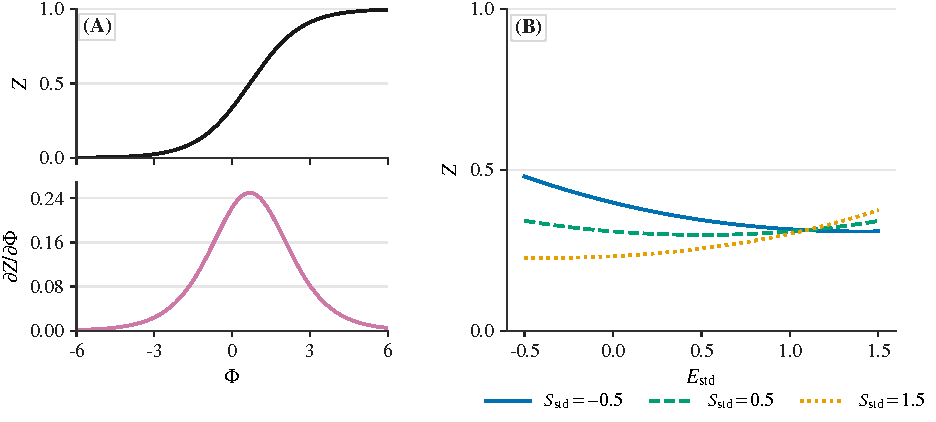
\includegraphics[width=0.315\linewidth,clip,trim={0bp 0bp 224.616bp 0bp}]{figure_1_phase_policy.pdf}%
  \hspace{0.02\linewidth}%
  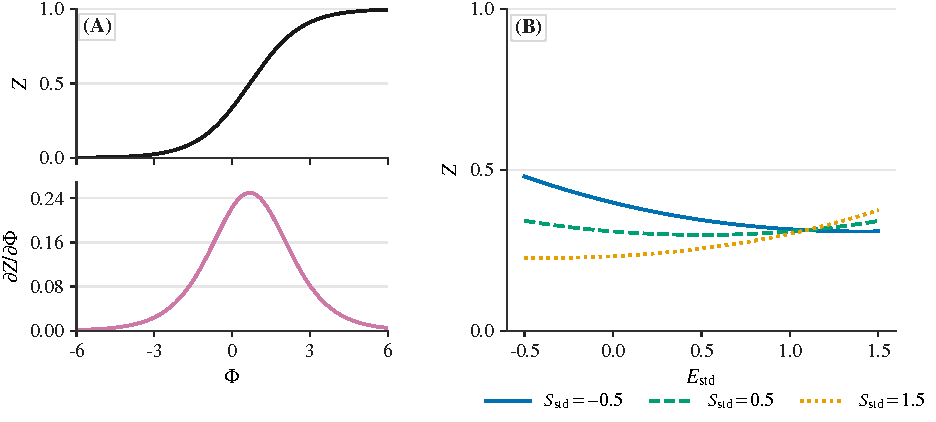
\includegraphics[width=0.315\linewidth,clip,trim={224.616bp 0bp 0bp 0bp}]{figure_1_phase_policy.pdf}

  \captionsetup{justification=justified,singlelinecheck=false}
  \caption{\textbf{Data scope:} model-implied bounded-response geometry under the fitted preprocessing and parameter contract (Figure~S4). \emph{(A)} shows $Z(\Phi)=\tfrac{Be^{\Phi}}{Be^{\Phi}+k}$ and local gain $\tfrac{\partial Z}{\partial \Phi}=Z(1-Z)$, which is largest near $Z\approx 0.5$ and attenuates in the tails. \emph{(B)} shows model-implied slices of $Z$ versus $E_{\mathrm{std}}$ for $S_{\mathrm{std}}\in\{-0.5,0.5,1.5\}$ at fixed high-stress settings ($T_{\mathrm{std}}=1.2$, $M_{\mathrm{std}}=0.8$, $D_{\mathrm{std}}=0.6$). \textbf{Method context:} this is an in-sample geometry diagnostic generated under the same bounded-domain contract as the paper figures; primary inferential evidence remains Tier A/B refit OOS leave-one-country-out evaluation (the primary spatial validation pathway), with rolling-origin serving as a temporal scope diagnostic. \textbf{Interpretation boundary:} read at the country--year state level under thin support (167 complete-case observations) with uneven regime coverage; descriptive, non-causal, and not a policy-optimization result.}
  \label{fig:phase-policy}
\end{figure}

Interactions and curvature induce regime dependence, so amplifier/suppressor labels are interpreted locally (conditionally) rather than globally. For example, if $\Phi$ contains an interaction $c_{ab}\,a\,b$, then the marginal effect of $a$ depends on $b$, and a quadratic term $c_{a2}a^2$ yields a state-dependent slope $\partial \log S/\partial a = c_a + 2c_{a2}a$. Consequently, a modifier can change sign across regimes.

Concretely, let $v$ denote a state consisting of the two structural drivers and all standardized contextual modifiers in \eqref{eq:phi}, i.e., $v=(X,Y,C_{\mathrm{std}},M_{\mathrm{std}},T_{\mathrm{std}},D_{\mathrm{std}},G_{\mathrm{std}},E_{\mathrm{std}},S_{\mathrm{std}},R_{\mathrm{std}})$.
For each modifier $j$, the local directional effect is computed as
\[
g_j(v)\;=\;\left.\frac{\partial \Phi}{\partial j_{\mathrm{std}}}\right|_{v},
\qquad\text{so that}\qquad
\left.\frac{\partial Z}{\partial j_{\mathrm{std}}}\right|_{v}=Z(v)(1-Z(v))\,g_j(v).
\]
A modifier $j$ is labeled as an \emph{amplifier} at state $v$ when $g_j(v)>0$ and as an \emph{suppressor} when $g_j(v)<0$. Under \eqref{eq:phi}, $g_j(v)$ reduces to $c_j$ for a pure main effect and becomes state-dependent under interactions and quadratic terms (e.g., $c_a+c_{ab}b$ or $c_a+2c_{a2}a$). These labels summarize directional structure in the fitted model and are not, by themselves, causal claims. In the fitted v2 model the terms that carry identified coefficients are the contextual channels $M$, $T$, $E$ and $R$, together with the interactions $c_{\mathrm{tr}}TR$ and $c_{\mathrm{yr}}Y_{\mathrm{s}}R$; the accelerator and buffer vocabulary below is retained as a way of reading the fitted signs, not as a claim that all eight originally proposed channels were estimated \parencite{McAdam1996,Putnam2000,Prior2007,Sunstein2018,TajfelTurner1979,MeltzerRichard1981,Coleman1988,Hastie2009ESL}.

\subsection*{Data preparation, bounded-domain mapping, and logit-space estimation}\label{sec:model-fitting}
The model in \eqref{eq:saturation} requires $X$ and $Y$ to be strictly positive and well-behaved under logs and fractional powers. The two structural drivers are mapped into a numerically stable interior interval $[\varepsilon,1-\varepsilon]$ using clipped min--max scaling:
\begin{equation}
\label{eq:x_map}
u_X=\mathrm{clip}_{[0,1]}\!\left(\frac{X_{\mathrm{raw}}-x_{\min}}{x_{\max}-x_{\min}}\right),\qquad
X=\varepsilon+u_X(1-2\varepsilon),
\end{equation}
\begin{equation}
\label{eq:y_map}
u_Y=\mathrm{clip}_{[0,1]}\!\left(\frac{Y_{\mathrm{raw}}-y_{\min}}{y_{\max}-y_{\min}}\right),\qquad
Y=\varepsilon+u_Y(1-2\varepsilon),
\end{equation}
with $\varepsilon$ set small (e.g., $10^{-4}$) to avoid endpoint logits and keep subsequent computations finite. Throughout, the clipping operator is defined as $\mathrm{clip}_{[0,1]}(u)=\min\{1,\allowbreak\max\{0,u\}\}$, ensuring $X,Y\in(\varepsilon,1-\varepsilon)$.
Contextual modifiers are supplied on a mix of curated index scales and raw measurement scales. Raw-scale modifiers are standardized as $j_{\mathrm{std}}=(j-\mu_j)/\sigma_j$, while already-indexed modifiers are used on their given scales, preventing unit-driven domination in $\Phi$ \parencite{Hastie2009ESL}.
A complete notation glossary and formal regime definitions are provided in Supplementary Tables~S15--S16.

Equation \eqref{eq:saturation} implies a convenient additive representation in log-odds space. From
\[
\frac{Z}{1-Z}=\frac{S}{k}=\frac{X^{\alpha}Y^{\beta}e^{\Phi}}{k},
\]
one obtains
\begin{equation}
\label{eq:logit}
\mathrm{logit}(Z)
=\log\!\left(\frac{Z}{1-Z}\right)
=\alpha\log X+\beta\log Y+\Phi-\log k.
\end{equation}
Equivalently, letting $B:=X^{\alpha}Y^{\beta}$ and $s:=\ln(B/k)$, one obtains the reduced-coordinate form
\[
Z=\sigma(\Phi+s),
\qquad \text{with ridge } Z=0.5 \;\Leftrightarrow\; \Phi+s=0,
\]
which makes explicit the mid-response boundary separating low-uptake and high-uptake regimes.
This reduced-coordinate geometry is visualized (Figure~\ref{fig:main-function-views}): constant-$Z$ contours are diagonals in the $(\Phi,s)$ plane and the ridge $Z=0.5$ delineates the most responsive band---a geometric consequence of the $[0,1]$-bounded mapping rather than an empirically discovered threshold. Away from this band the mapping saturates ($Z\to 0$ or $Z\to 1$), attenuating marginal effects.

\begin{figure}[!htbp]
  \centering

  \newcommand{\FigureFiveCaption}{\textbf{Data scope:} reduced-coordinate geometry of the main function $Z=\sigma(\Phi+s)$ with $s:=\ln(B/k)$ (where $B=X^{\alpha}Y^{\beta}$) (Figure~S5). Values are computed in the interior band $(\varepsilon,1-\varepsilon)$ (here $\varepsilon=10^{-4}$), while the color scale is labeled by the conceptual endpoints $Z\in[0,1]$. \emph{(A)} Heatmap of $Z$ over $(\Phi,s)$ with constant-$Z$ contours and the ridge $Z=0.5$. \emph{(B)} Slices $Z(\Phi)$ at three shifts (low/baseline/high). \emph{(C)} Isometric surface of $Z(\Phi,s)$ with ridge and baseline slice overlaid. \textbf{Method context:} this is an in-sample geometry diagnostic; protocol interpretation is anchored to Tier A/B refit OOS leave-one-country-out evidence (the primary spatial validation pathway), with rolling-origin serving as a temporal scope diagnostic. \textbf{Interpretation boundary:} read as model-implied country--year geometry under thin support (167 complete-case observations) with uneven regime coverage; support-conditioned, non-causal, and not a transportability claim. The ridge at $Z=0.5$ is a geometric property of the bounded-scale mapping (maximum of $Z(1-Z)$), not an independently validated behavioral threshold.}

  \refstepcounter{figure}
  \addcontentsline{lof}{figure}{\protect\numberline{\thefigure}{\FigureFiveCaption}}
  \label{fig:main-function-views}

  \begin{tikzpicture}
    \node[inner sep=0] (img) {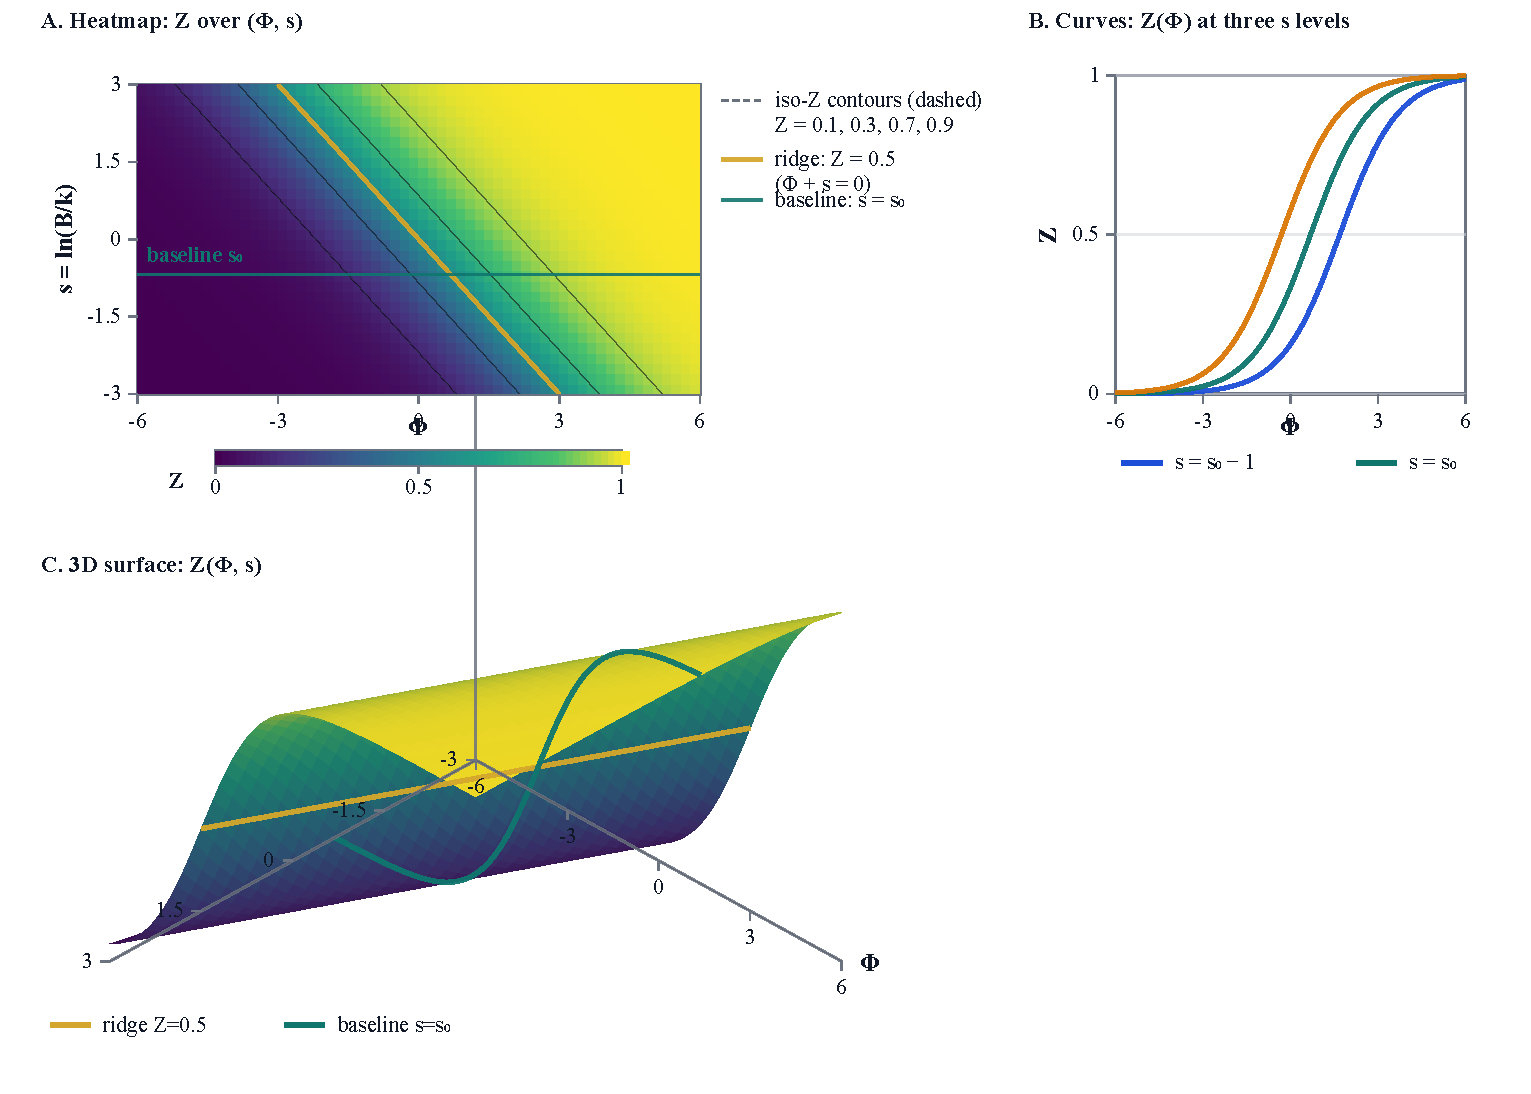
\includegraphics[width=\linewidth,height=0.74\textheight,keepaspectratio,trim={0 1.8cm 0 0.6cm},clip]{figure_2_main_function_geometry.pdf}};
    \begin{scope}[x={(img.south east)}, y={(img.north west)}]
      \node[
        anchor=north west,
        text width=0.39\linewidth,
        inner sep=0pt,
        outer sep=0pt
      ] at (0.63,0.47) {{\footnotesize\begin{minipage}{\linewidth}\setlength{\parindent}{0pt}\noindent\justifying\textbf{Figure~\thefigure.}~\itshape\FigureFiveCaption\end{minipage}}};
    \end{scope}
  \end{tikzpicture}
\end{figure}

This transformation motivates estimation on the logit scale: multiplicative exposure and contextual amplification/suppression become additive components, improving numerical conditioning and interpretability \parencite{McCullaghNelder1989}. When the observed outcome is stored on an unconstrained scale, it is mapped to the same interior interval $[\varepsilon,1-\varepsilon]$ before taking logits, using the same clipped min--max principle as in \eqref{eq:x_map}--\eqref{eq:y_map}.

\begin{equation}
\label{eq:z_map}
u_Z=\mathrm{clip}_{[0,1]}\!\left(\frac{Z_{\mathrm{raw}}-z_{\min}}{z_{\max}-z_{\min}}\right),\qquad
Z=\varepsilon+u_Z(1-2\varepsilon).
\end{equation}

Parameters $\theta=(\alpha,\beta,k,\phi_0,\{c_\cdot\})$ are estimated by minimizing a composite objective that balances accuracy, rank-consistency, calibration bias, and regularization:
\begin{equation}
\label{eq:loss}
\mathcal{L}(\theta)=(1-R^2)+(1-\mathrm{Corr})+\mathrm{MAE}+w_b|\mathrm{Bias}|+\lambda\|\theta\|_2^2,
\end{equation}
where $\lambda>0$ controls ridge shrinkage. Regularization is used because macro-social indicators are correlated, and the interaction structure in \eqref{eq:phi} can otherwise induce unstable estimates and poor out-of-sample behavior \parencite{Hastie2009ESL,Greene2018Econometric}. Parameters are constrained to plausible ranges to avoid degenerate saturation and to keep the exposure elasticities interpretable:
\[
\alpha,\beta\in[0.01,2.0],\quad k\in[0.1,10],\quad \phi_0\in[-10,10],\quad c_\cdot\in[-5,5].
\]
During evaluation, $\Phi$ is clamped to a wide symmetric interval to prevent overflow in $\exp(\Phi)$,
\begin{equation}
\label{eq:phi_clamp}
\Phi \leftarrow \mathrm{clip}_{[-50,+50]}(\Phi),
\end{equation}
without materially affecting inference in the empirically relevant region. The boundedness of $Z$ is implied by \eqref{eq:saturation}; the clamps and interior mapping help ensure stable computation of $S$ and $\mathrm{logit}(Z)$.

Because the objective in \eqref{eq:loss} is non-convex under the full interaction structure, estimation uses a hybrid strategy: a global evolutionary stage followed by bounded quasi-Newton refinement under box constraints \parencite{StornPrice1997,NocedalWright2006}. To reduce sensitivity to local minima, the evolutionary stage is run with multiple randomized initial populations, and the best candidates are refined using bounded quasi-Newton line-search updates under the same box constraints. Convergence is assessed on relative objective improvement and parameter stability; the reported solution is the best feasible candidate across restarts.

Evaluation adopts an explicit bounded-domain contract consistent with Eqs.~\eqref{eq:x_map}--\eqref{eq:z_map}. The canonical country--year panel comprises 76 countries and 167 complete-case observations spanning 1990--2023; each row is a unique $(\mathrm{iso3},\mathrm{year})$ and defines the support envelope for interpretation. Let $\varepsilon=10^{-4}$ and define the interior band $\mathcal{I}_\varepsilon=[\varepsilon,\,1-\varepsilon]$. Structural drivers and the observed outcome are mapped into $\mathcal{I}_\varepsilon$ using the clipped min--max contract; for evaluation, panel bounds are set to $(x_{\min},x_{\max})=(0.3304,0.9544)$ and $(y_{\min},y_{\max})=(-1.6078,3.4280)$, and outcome normalization bounds are set to $(z_{\min},z_{\max})=(\num{-1.6094638811769215},\,\num{1.5846349235822439})$. These are the realised v2 ranges; the earlier window excluded six observations and clamped them to the floor of the interior band.

Under this contract, predictions $\widehat{Z}$ are computed by applying \eqref{eq:saturation} row-wise and clamping to $\mathcal{I}_\varepsilon$ to avoid endpoint logits; residuals are defined on the bounded scale as $e_i=Z_i-\widehat{Z}_i$. Evaluation reports association and error-scale summaries ($R^2$, $\mathrm{Corr}$, MAE, RMSE, Bias) together with calibration and residual diagnostics, and assesses robustness via temporal splits and structural ablations of $\Phi$ while holding fitted coefficients fixed. All transformations are deterministic and fully specified by the reported bounds and $\varepsilon$; values outside the evaluation bounds are projected to the nearest interior point through the clipped min--max contract. Monotonicity preserves rank order within bounds, and numerical stability is enforced through interior-band logits and bounded exponentials (Eq.~\eqref{eq:phi_clamp}). Optimization uses fixed budgets and termination tolerances so that convergence behavior is reproducible given the same data and bounds. Any inspection query outside $(x_{\min},x_{\max})\times(y_{\min},y_{\max})$ is projected to the nearest interior point before computing $S$ and $Z$, so exported surfaces do not present unsupported extrapolation. The same contract keeps evaluation, figure generation, and interactive inspection aligned to a single auditable mapping, reducing the risk of silent drift between scripts. Because the contract is applied symmetrically to observed outcomes and model predictions, error metrics remain interpretable on a common bounded scale. When uncertainty summaries are reported, they are transformed through the same saturation map and truncated to $\mathcal{I}_\varepsilon$, so intervals respect the modeled support. This explicit scoping clarifies that reported effects are conditional on the empirical support of the panel and should not be interpreted as extrapolations beyond the observed driver ranges. Domain violations are therefore handled transparently via clipping rather than being silently propagated through logs, powers, exponentials, and logits. Together, these guarantees make boundary behavior auditable, keep cross-section, temporal-split, and ablation comparisons on the same numerical support, and ensure that residuals, calibration summaries, and exported surfaces can be regenerated from identical bounded inputs without ambiguity about preprocessing or numerical guards.

\section{Evaluation and Uncertainty Quantification}
Evaluation uses the canonical country--year panel and the bounded-domain preprocessing contract specified in the Method section. Let $\widehat{Z}$ denote predictions on the bounded evaluation scale and define residuals $e_i=Z_i-\widehat{Z}_i$. In inferential prioritization, Tier A/B statements are treated as primary only when supported by refit out-of-sample checks; in-sample fit is reported as descriptive context. Performance is summarized with complementary association- and error-scale diagnostics,
\begin{equation}
\label{eq:eval_metrics_r2_corr}
R^2 = 1-\frac{\sum_i e_i^2}{\sum_i (Z_i-\overline{Z})^2},\qquad
\mathrm{Corr}(Z,\widehat{Z})=\frac{\sum_i (Z_i-\overline{Z})(\widehat{Z}_i-\overline{\widehat{Z}})}
{\sqrt{\sum_i (Z_i-\overline{Z})^2}\sqrt{\sum_i (\widehat{Z}_i-\overline{\widehat{Z}})^2}},
\end{equation}
\begin{equation}
\label{eq:eval_metrics_errors}
\mathrm{MAE}=\frac{1}{n}\sum_i |e_i|,\qquad
\mathrm{RMSE}=\sqrt{\frac{1}{n}\sum_i e_i^2},\qquad
\mathrm{Bias}=\frac{1}{n}\sum_i e_i.
\end{equation}
Cross-validation diagnostics are computed first at row level on the canonical panel and then additionally summarized on support-collapsed unique $(\mathrm{iso3},\mathrm{year})$ aggregates to separate replication-heavy weighting from effective support diagnostics. The authoritative protocol artifacts are the country-out artifact, the rolling-origin artifact, the parameter-stability artifact, the interval-coverage artifact (protocol/tier coverage summaries), and the lockbox artifact (release-gated frozen-split lockbox confirmation).
Within these protocol artifacts, the refit metric family carries primary inferential weight, including \texttt{testMetricsRefit} and \texttt{aggregatesRefit} together with their support-collapsed counterparts. Canonical fixed-model counterparts, including \texttt{testMetricsCanonical} and \texttt{aggregatesCanonical}, are retained as descriptive diagnostics only.
Headline fit on the bounded evaluation scale (Eq.~\eqref{eq:z_map}) is reported for the full canonical panel (Table~\ref{tab:panel_fit_headline}). Association is relatively high, but the mean residual bias is negative, indicating systematic over-prediction in the normalized band ($\widehat{Z}>Z$ on average). Consequently, interpretation emphasizes calibration and uncertainty-aware diagnostics over any single global fit statistic. Support-aware checks on the same bounded scale are provided in Figure~\ref{fig:eval-pair} and Figure~S9, including observed-versus-predicted values with hexagonal support density, decile-wise calibration summaries, and residual diagnostics that separate bias from dispersion.

Because the canonical panel is intentionally unbalanced (irregular year coverage by country and uneven completeness across the modeled variable block), evaluation is interpreted conditional on observational support: where the data are sparse, surface geometry may reflect extrapolation or saturation rather than evidenced structure. Robustness is assessed deterministically by recomputing the same bounded-scale metrics under controlled perturbations without refitting coefficients; these robustness tables are fixed-model descriptive diagnostics and are not interpreted as replacements for refit OOS protocol evidence. Temporal stability is examined via empirical year tertiles (cut years 2006 and 2012; Table~S12), and structural ablations isolate the incremental contribution of interaction and quadratic components of $\Phi$ ((i) main terms only, (ii) main plus interactions, (iii) full specification including quadratics). These checks are summarized (Table~S5) and are interpreted as descriptive evidence about regime geometry (interaction-driven narratives) rather than as marginal gains in $R^2$. Country-level heterogeneity is examined by recomputing bounded-scale metrics within each country’s observed years; because within-country variance in $Z$ can be small for short series, $R^2$ may be unstable and error-scale diagnostics are emphasized. Among countries with at least 30 observations, RMSE has median \num{0.0878} with interquartile range \num{0.0699}--\num{0.0971}. These slice-wise summaries motivate two constraints carried into the visual layer: regime narratives are paired with explicit coverage diagnostics, and calibration is treated as distributional (support-aware) rather than as a single global slope.

Uncertainty quantification is treated as a robustness envelope for the fitted mapping rather than as a fully parametric stochastic error model. Repeated resampling provides uncertainty bands for global performance and fitted parameters \parencite{EfronTibshirani1993Bootstrap, DavisonHinkley1997Bootstrap}, reported for the fitted specification (Table~S6). In the visual analytics layer, uncertainty is propagated to response-surface and sensitivity views using resampling-based envelopes with country-level clustering where refits are required \parencite{cameron2015practitioner}. For any fixed input configuration $\mathbf{x}_0$, prediction intervals are reported as empirical quantiles of $\widehat{Z}^{(b)}(\mathbf{x}_0)$ (Eq.~\eqref{eq:pred_interval_eval}), keeping uncertainty on the same bounded scale used for evaluation and visualization. In the executable Phase-1 pipeline, the interval-coverage artifact is produced from fold-level empirical residual-quantile-shifted intervals (primary) with a symmetric Gaussian residual comparator and then aggregated by protocol/tier/support regime; this artifact is the authoritative coverage object for Gate-3 reproducibility checks. Observed 95\% coverage is materially below nominal in rolling-origin folds (Tier A~=~57\%, Tier B~=~31\%, Tier C~=~24\%) and in higher-complexity specifications, confirming that rolling-origin serves as a temporal scope diagnostic rather than a validation pathway for headline claims. These interval summaries are interpreted as protocol-specific, support-conditioned, and regime-dependent uncertainty descriptors rather than universal validity guarantees.

\begin{equation}
\label{eq:pred_interval_eval}
\widehat{Z}^{(b)}(\mathbf{x}_0)=f(\mathbf{x}_0;\widehat{\theta}^{(b)}),\qquad
\mathrm{PI}_{0.95}(\mathbf{x}_0)=\bigl[q_{0.025}\{\widehat{Z}^{(b)}(\mathbf{x}_0)\},\;q_{0.975}\{\widehat{Z}^{(b)}(\mathbf{x}_0)\}\bigr],
\end{equation}

To assess whether interval behavior varies by predicted-$Z$ regime, the 167 panel observations were stratified into three predicted-$Z$ tertiles (low: $\hat{Z}<0.33$; mid: $0.33\le\hat{Z}<0.67$; high: $\hat{Z}\ge 0.67$). Under the LOO country-out protocol, coverage is closest to nominal in the transition corridor (mid tertile) and falls below nominal in the saturated tails, consistent with the compression effects of the bounded mapping: narrow intervals in low-$Z$ and high-$Z$ regimes reflect local flatness of the sigmoidal transform rather than strong parameter identification. Regime-stratified coverage summaries are tabulated in Table~S20; regime-stratified calibration under rolling-origin folds is flagged as a priority validation extension (see Limitations and extensions, Section~8).

\subsection*{Collinearity in the retained block}\label{sec:collinearity}
Pearson correlations on complete-case rows contextualize collinearity in the modeled variable block (Figure~S11), and variance inflation factors provide a complementary screen (Table~S13). The screen is not decorative: two of the six retained covariates are substantially dependent on the others. Welfare capacity $R$ reaches $\mathrm{VIF}=\num{9.19}$ and education capacity $E$ reaches $\mathrm{VIF}=\num{4.74}$, while the remaining four sit between \num{1.08} and \num{3.09}.

The dependence has an identifiable source, and it is not a coding error. $R$ is an affine rescaling of the Human Development Index---$R = \num{7.303771}\,\mathrm{HDI} - \num{6.005361}$, with maximum residual $\num{0.000000}$ over \num{13441} upstream rows---and HDI is itself partly an education measure, so $R$ and $E$ (gross secondary enrolment) share a component by construction. A model that carries both is not fitting two independent channels. Coefficients on $R$ and $E$ are therefore reported as conditional associations under this design; the paper does not claim to separate their individual contributions, and no conclusion rests on doing so. The shock channel is unaffected and is in practice orthogonal to the rest ($\mathrm{VIF}=\num{1.08}$). Because the dependence is real, the question is whether to engineer it away. Dropping $R$ would take the maximum VIF from \num{8.74} to \num{2.49} at a cost of \num{0.0029} of in-sample $R^2$, and would actually \emph{raise} grouped $k$-fold from \num{0.4235} to \num{0.4401} for Tier~A and from \num{0.4827} to \num{0.5081} for Tier~B. That improvement is the reason not to take it. $R$ entered the design before any of these numbers existed, for a Meltzer--Richard reason about welfare-state capacity; removing it after observing that the fit improves is post-hoc specification selection, and a model tuned against the evaluation it reports cannot then be judged by that evaluation. The dependence is therefore disclosed rather than engineered away, and the cost of disclosing it is stated plainly: no argument in this paper rests on the size of $c_R$.

Removing the two dependent channels does cost real explanatory power---in-sample $R^2$ falls from \num{0.4728} to \num{0.4100}---which is the honest reason to keep them: they carry signal, just not separable signal.

\begin{figure}[!htbp]
  \centering
  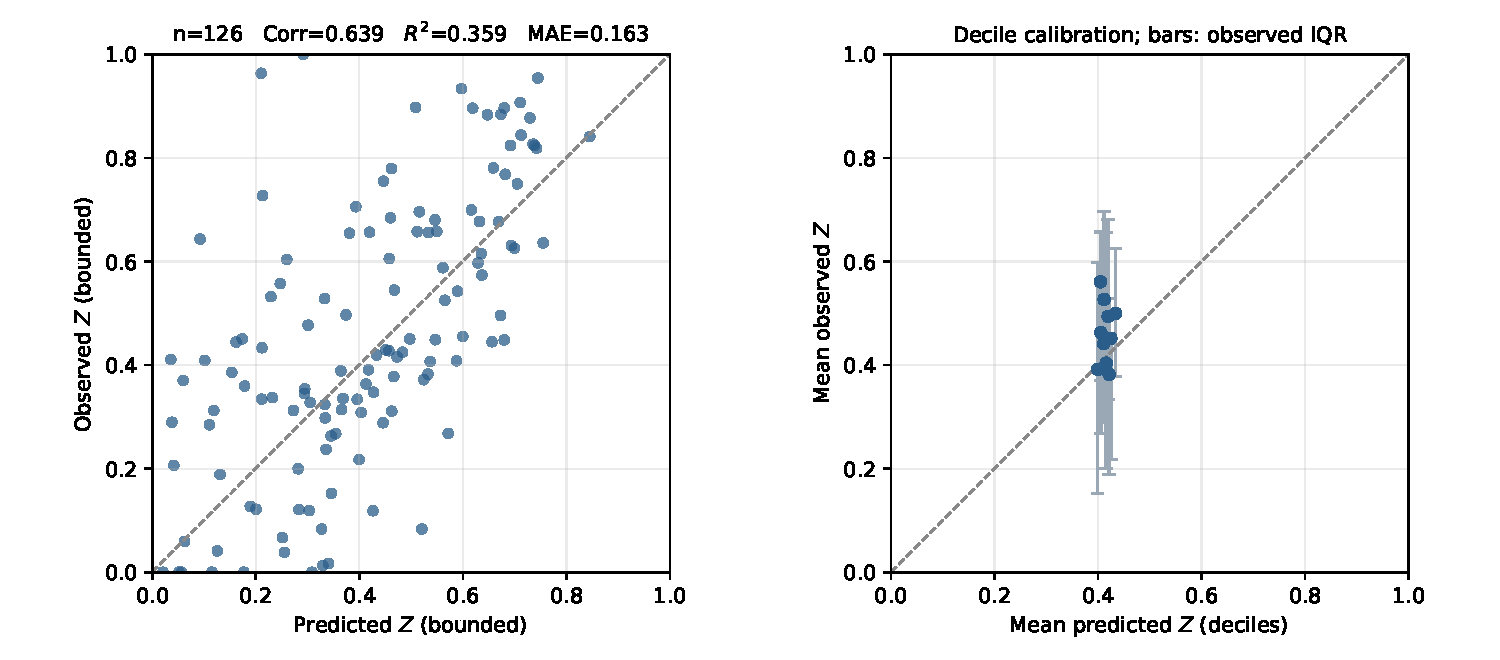
\includegraphics[width=\linewidth]{fig_eval_pair.pdf}
  \caption{\textbf{Data scope:} bounded-scale in-sample fit and decile-calibration diagnostics on the canonical v2 panel (167 complete-case observations). Observed outcomes $Z$ and predictions $\widehat{Z}$ are evaluated on the same bounded scale $\mathcal{I}_\varepsilon=[\varepsilon,1-\varepsilon]$ with $\varepsilon=10^{-4}$. \textbf{Method context:} the left panel shows observed-versus-predicted values with hexagonal support density; the right panel reports decile-wise mean $Z$ and within-decile IQR conditional on predicted level. \textbf{Interpretation boundary:} this figure provides descriptive fit context only; primary inferential weight remains Tier~A/B refit OOS evidence (Section~5), and the figure does not by itself support causal or policy claims.}
  \label{fig:eval-pair}
\end{figure}

\section{Visual Analytics Tooling}
Visual analytics is treated as an auditable extension of the estimation pipeline, not as post-hoc illustration. The objective is to make the bounded nonlinear response map (Eqs.~\ref{eq:core}--\ref{eq:saturation}), the contextual field (Eq.~\ref{eq:phi}), and the preprocessing contract (Eqs.~\ref{eq:x_map}--\ref{eq:y_map}) directly interrogable under the same bounded-domain assumptions used for fitting and evaluation. Because the country--year panel is intentionally unbalanced, the tooling enforces a provenance chain (canonical extract $\rightarrow$ preprocessing $\rightarrow$ fitted coefficients $\rightarrow$ deterministic export) and pairs empirical-support diagnostics with functional-geometry examination to reduce the risk of (i) reading smooth surfaces as uniformly supported and (ii) translating coefficient signs into global narratives in a regime-dependent mapping \parencite{ThomasCook2005IlluminatingPath,Keim2010MasteringVisualAnalytics,MacEachren2005VisualizingUncertainty}. In practical terms, each view is anchored to the decomposition implied by the model: analysts can move from raw driver settings to the implied contextual contribution ($\Phi$), to exposure and saturation geometry (Eqs.~\ref{eq:core}--\ref{eq:saturation}), and back to the empirical evidence that underwrites those settings, rather than treating any single plot as self-sufficient. This ``round-trip'' analysis loop is designed to help keep readings faithful to the bounded mapping: leverage statements are anchored in where the system sits on the saturating curve (Eq.~\ref{eq:saturation}), and contextual statements are grounded in the realized $\Phi$ field (Eq.~\ref{eq:phi}) under the same preprocessing contract used everywhere else (Eqs.~\ref{eq:x_map}--\ref{eq:y_map}). Concretely, the UI provides response-surface views with pinned probing and paired 3D/2D companions so that saturation shoulders and regime transitions are observable under the saturating transform (Eq.~\ref{eq:saturation}) and the same numerical safety contract used for production exports (Eq.~\ref{eq:phi_clamp}) (Figures~S13--S14). These coordinated views are coupled with explicit coverage cues (e.g., density overlays and ``where-data-exist'' annotations) so that surface interrogation remains conditioned on observed country--year support, especially near regime boundaries where slopes are highest. This complements the reduced-coordinate explanation (Figure~\ref{fig:main-function-views}) and is summarized for policy-facing synthesis via a deterministic phase/leverage view (Figure~\ref{fig:phase-policy}) generated under the same bounds in Eqs.~\ref{eq:x_map}--\ref{eq:y_map} and a fixed coefficient source (the coefficient module). An optional ``AI Interpreter'' module can be enabled to send a JSON snapshot of the current parameter state and model decomposition (including $Z$ and $\Phi$) to an external LLM service to draft a brief note, but it is not required for reproducibility, does not alter deterministic computation, and is not used to generate any reported coefficients, figures, or numerical claims.

Uncertainty is framed as a first-class visual object rather than as a footnote: interval summaries are centralized (coefficient forest plot, Figure~S2) and the application assembles aligned, non-redundant diagnostics (e.g., calibration and residual checks; temporal and country slices) together with ablation and numerical-sensitivity summaries for stability parameters that affect the bounded transform (including the interior-band offset and the $\Phi$ clamp). The intent is not to ``add error bars'' after the fact, but to make uncertainty commensurate with mechanism: the same scenario and surface questions posed to the point estimate can be re-asked against envelope summaries, so that visually salient patterns are retained only if they are stable across plausible refits or perturbations. Outputs are schema-versioned to support an auditable evidence-bundle workflow in which readers can reference diagnostics without duplicating the full interactive report, while an auditor can trace claims to deterministic artifacts through the PDF export pathway (Figure~S15). Crucially, exports bind the narrative to concrete artifacts (view state, parameter state, and the bounded-domain contract) so that reported figures remain traceable to the same reproducible pipeline that generated the evaluation metrics. Across the tooling, empirical-support views are consulted before mechanism views, and mechanism views before policy narratives; where the panel is thin or predictors are correlated, reading emphasizes local leverage and regime transitions rather than global causal language, and where the bounded map saturates, the analysis relies on sensitivity views rather than linear slope intuition, keeping the narrative aligned with what the observed country--year data can support and turning each exported view into a checkable claim rather than an illustrative sketch \parencite{Keim2010MasteringVisualAnalytics,MacEachren2005VisualizingUncertainty,Peng2011Reproducible}.

\needspace{6\baselineskip}
\section{Results}
Results are reported for the fitted bounded structural model under the same preprocessing and numerical-safety contract used for estimation and evaluation (Eqs.~\eqref{eq:core}, \eqref{eq:phi}, and \eqref{eq:saturation}; Section~5). To distinguish primary evidence from exploratory sensitivity, results follow a strict tiered structure: Tier A/B are supported by refit out-of-sample validation (country-out as the primary spatial validation pathway; rolling-origin as a temporal scope diagnostic) and carry primary inferential weight, while Tier C is retained as exploratory sensitivity and is excluded from headline inferential claims. A frozen lockbox holdout check is reported separately from development CV and is used as a release-gated confirmation layer for final headline interpretation when protocol checks pass. Global agreement with the canonical panel on the bounded outcome scale is summarized in Table~\ref{tab:panel_fit_headline} (Figure~\ref{fig:eval-pair}); these in-sample diagnostics are descriptive context, while strong inferential statements are anchored to Tier A/B out-of-sample protocol evidence. Interpretation is explicitly conditioned on empirical support in the canonical panel (Table~S2; Figure~\ref{fig:data-funnel}): with 167 complete-case observations and support-per-parameter ratios of 15.18/9.28/7.59 (Tier A/B/C), high-dimensional terms are support-constrained and broad generalization claims are not warranted.

To orient the reader, the Results section is organized as an evidence roadmap. First, out-of-sample validation under refit protocols (Key findings 0) is reported as the primary empirical anchor. Next, regime geometry and state-dependent leverage (Key findings I) are summarized as model-implied properties of the bounded map, paired with support-aware diagnostics. Finally, the most robust contextual patterns in $\Phi$ (Key findings II) are summarized, emphasizing stability across folds and treating higher-order terms as exploratory components of the fitted surface rather than stand-alone mechanisms.
Across all Results subsections, regime-level interpretation is conditioned on the same thin-support envelope (167 complete-case observations with uneven low/mid/high regime density), and should be read as support-conditioned model geometry rather than universal regularity.

For auditability, primary out-of-sample evidence and support diagnostics are anchored to Table~S2 (country--year support and fold artifacts), while the tier hierarchy and classification thresholds are summarized in Table~S0. Instability and fold-level caveats are logged in the supplementary instability/failure log, and all interpretive statements in this section are conditioned on the same support structure (Table~S2) and diagnostics referenced in the supplementary.

\subsubsection*{Key findings 0: Out-of-sample validation results under refit protocols}

Primary inferential weight is placed on \emph{repeated grouped $k$-fold} cross-validation: countries are assigned to folds as whole units, so no country appears in both train and test, and $k=5$ folds are drawn $20$ times for $100$ held-out evaluations. This replaces leave-one-country-out (LOO) as the primary spatial protocol, for a measured reason. With 167 rows across 76 countries, a country-out fold holds out between one and four rows; $R^2$ is undefined below three pairs, so 36 of the 48 folds carry no $R^2$ at all and the reported per-fold median describes the twelve survivors rather than the model (KI-14). Grouped $k$-fold keeps the same spatial separation while giving every fold roughly seventeen test rows, and the twenty repeats make the reported statistic a distribution rather than one arbitrary split.

Under this protocol, in-sample-to-out-of-sample degradation is modest and the tier ordering does not survive it. Median held-out $R^2$ is \num{0.4063}/\num{0.4767}/\num{0.4802} for Tier A/B/C (interquartile ranges \num{0.122}--\num{0.519}, \num{0.115}--\num{0.551}, \num{0.106}--\num{0.534}), against an in-sample $R^2$ of \num{0.2516} on the same rows: held-out performance now matches or exceeds in-sample fit, and the fold-to-fold dispersion is markedly narrower than on the 87-cell panel. Median held-out RMSE is \num{0.1835}/\num{0.1781}/\num{0.1780} (IQR \num{0.1679}--\num{0.2283}, \num{0.1638}--\num{0.2118}, \num{0.1627}--\num{0.2268}). The three tiers remain statistically indistinguishable once countries are held out: Tier C exceeds Tier A both in-sample (\num{0.5642} against \num{0.4728}) and out of sample (\num{0.4802} against \num{0.4063}), but the out-of-sample gain is \num{+0.0035} over Tier B against \num{+0.0914} in sample, and it changes sign across seeds. Added complexity buys almost no transfer, which is why Tier C is reported as exploratory.

The fixed production coefficients are evaluated on the same folds and behave differently by tier: median held-out $R^2$ is \num{0.2407}/\num{0.3066}/\num{0.2523} (IQR derived from the artifact). Tier A's canonical family is still the weakest, but its lower quartile is now positive (\num{0.123}); Tiers B and C transfer better as fixed maps than they do when refitted per fold. This split is reported rather than smoothed: the production coefficients are not the fold-refit optimum, and the difference is largest exactly where the model is simplest.

Leave-one-country-out is retained as a \emph{spatial stress test}, not as the primary evidence. Across its 70 folds median held-out RMSE is \num{0.1506}/\num{0.1449}/\num{0.1369}, and because each fold holds out one country the pooled held-out series can still be assembled: predicting every row exactly once yields pooled $R^2$ of \num{0.4056}/\num{0.4629}/\num{0.4420} (refit) and \num{0.2601}/\num{0.3239}/\num{0.2516} (canonical) over all 167 rows. That the pooled statistic is positive while the per-fold median is negative is the whole point: the negative median was an artefact of computing a variance ratio on one to four points, not a finding about the model.

Forward-chaining rolling-origin evaluation serves as a complementary temporal scope diagnostic. Across 20 folds, median out-of-sample RMSE is \num{0.1296}/\num{0.1419}/\num{0.1465}, comparable to the spatial errors. Parameter sign consistency is reported per coefficient rather than as a blanket threshold. Across the country-out protocol every coefficient keeps its sign in at least 0.75 of folds, and the artefact marks the two weakest Tier B terms ($x_{\text{safe}}$, $y_{\text{safe}}{:}r$) as unstable at the 0.80 threshold rather than claiming stability the sample cannot support.


\subsubsection*{Key findings III: what the bounded form buys, and what it costs}\label{sec:functional-form}

The comparison that matters most for this paper's claim is not between tiers but between functional forms. Both models below are fitted to the same 167 rows with the same six covariates ($X$, $Y$, $T$, $E$, $R$, $M$) and evaluated on identical folds; the only difference is the link. The linear model is ordinary least squares; the bounded model wraps the same covariates in the saturation map. Source artifact: the functional-form artifact.

\begin{table}[!htbp]
\centering
\TableStyle
\caption{\textbf{Data scope:} 167 complete-case country--year observations, 76 countries, 1990--2023. \textbf{Method context:} identical rows, identical covariates, identical folds; the linear baseline is ordinary least squares, the bounded model is the paper's production map refitted per fold. \textbf{Interpretation boundary:} this tests the link function, not the construct audit; a near-tie at this sample size is the finding, and neither model's held-out fit supports a claim of predictive superiority.}
\label{tab:functional-form}
\begin{tabularx}{\linewidth}{@{}lrrr@{}}
\toprule
Model & In-sample $R^2$ & k-fold $R^2$ & Pooled LOO $R^2$ \\
\midrule
Ordinary linear regression          & \num{0.4618} & \num{0.4006} & \num{0.3871} \\
Saturating bounded map (this paper) & \num{0.2516} & \num{0.4063} & \num{0.4056} \\
\bottomrule
\end{tabularx}
\end{table}

The result is a near-tie, and the honest reading is narrower than either "the bounded form works" or "the bounded form fails". In sample the linear model is clearly better ($R^2=\num{0.4618}$ against \num{0.2516}): curvature costs accuracy where the data are dense. Out of sample the two are indistinguishable, with the bounded form ahead by \num{0.0057} under grouped $k$-fold (\num{0.4063} against \num{0.4006}) and by \num{0.0185} in the pooled country-out series (\num{0.3853} against \num{0.3871})---differences far inside the interquartile ranges (\num{0.1500}--\num{0.5011} for linear, \num{0.1552}--\num{0.5179} for bounded).

An earlier draft asserted that the linear baseline won decisively ($R^2$ \num{0.2020} against \num{0.1023}). That comparison could not be regenerated from the tree, and when the baseline is actually fitted on the canonical panel the gap does not appear. We report the measured values and withdraw the stronger claim. The corrected version supports only what the data support: at 167 country-years, the choice between these two links is not identified by predictive performance.

Two properties of the data explain why curvature does not pay. First, the pooled outcome is close to normally distributed with standard deviation $0.97$. A sigmoid's steepest gradient sits at its midpoint and decays in the tails; regressing a roughly linear outcome on it forces the curvature into the densest region and flattens exactly where the extremes lie. Second, two cells sit far outside the bulk---CHN 1990 at $Z=+3.37$ and IDN 2006 at $Z=-2.19$. Under min--max scaling they compress the other 85 rows into roughly $[0.22, 0.78]$; percentile anchoring recovers part of that range, but not a ranking between the models.

The bounded form was adopted because the outcome is a composite index on a closed scale. That argument concerns \emph{measurement}, not \emph{response shape}, and this sample does not arbitrate the shape. Nothing in 167 country-years indicates that effects flatten at high exposure. The manuscript accordingly makes no saturation claim; the transition-ridge behaviour discussed in Section~4 and illustrated in the visual analytics layer is a property of the fitted map, which is a different statement.

\emph{Fixed-coefficient comparison.} The refit metrics above train a model per fold. Evaluating the \emph{production} coefficients on the same held-out rows yields a negative coefficient of determination (Tier A $R^2=-2.01$, Tier B $-0.97$, Tier C $-0.90$; RMSE 0.190). A negative value means the fixed model predicts held-out countries worse than those countries' own mean. This is expected once the outcome is no longer a rescaling of a predictor: the coefficients describe population-level associations and do not transport to unseen countries at this sample size. We report it because suppressing it would misrepresent the cross-national transferability of the fitted map.

Under the rolling-origin protocol, 12 forward-chaining folds are generated, each training on survey years up to a cut point and evaluating the next survey year (2007 through 2022). Median out-of-sample RMSE across those folds is \num{0.1296}/\num{0.1419}/\num{0.1465} for Tier A/B/C, comparable to the country-out errors. Because each fold holds out a single survey year, per-fold test sets are small; the protocol is reported as a \emph{temporal scope diagnostic}, and rolling-origin coverage at the 95\% nominal level is not emphasised for the same reason.

\emph{Lockbox protocol status.} The lockbox split is generated deterministically (20\% of cells, cycle \texttt{2026Q4-R4}) and reserves 17 country--years across 11 countries at one to three observations each. Because those 17 cells are few and thinly spread, a lockbox evaluation tests cross-national transport with very little per-country support; the confirmation metrics are therefore reported as a held-out descriptive check, not as confirmation of transferable effects. No claim in this paper rests on lockbox performance.

The scope of that protection needs stating precisely, because the panel grew after the split was drawn. The 17 reserved cells remain reserved and remain excluded from development. The additional 59 country--years came from covariate backfills, and the equivalence constants that make those backfills valid were estimated on the panel rows that already existed---that is, on development data. The recovered cells are out of sample in the cross-validation sense only; they are not blind in the lockbox sense. This is a real limitation and it is disclosed rather than papered over: the recovered cells are the ones with the sparsest covariate coverage, so they are on average harder targets, but hardness is not blindness. Regenerating the split would restore full coverage at the cost of discarding the pre-registration, so the split is left in place.

Tier C (full exploratory complexity) is retained as an exploratory appendix, and the reason is a measured one rather than a convention. In sample, fit rises monotonically across the ladder---\num{0.4728}, \num{0.5549}, \num{0.5642} for Tiers A, B and C---so eleven extra parameters do buy in-sample $R^2$ (\num{+0.0837} over Tier A). Out of sample the picture is very different. Under repeated grouped $k$-fold the eleven extra parameters buy \num{+0.0035} over Tier B (\num{0.4802} against \num{0.4767}) while buying \num{+0.0914} in sample---an exchange rate of roughly 26 to 1---and that small positive difference is itself unstable: the median of Tier C's 200 within-seed repeats sits \emph{below} the median of Tier B's (\num{0.4585} against \num{0.4827}), the median difference is \num{-0.0061}, and the sign flips on roughly half of individual repeats. On 167 country-years, in-sample fit is not a guide to out-of-sample fit, and a model that appears to improve with complexity is not thereby better. We keep the tier and report that gap instead of deleting it, because the gap is the evidence. Tier C carries the support-risk flag, its inferential role is \texttt{exploratory}, and no headline claim rests on it; those properties are enforced by a test, so a future regeneration cannot quietly promote it.

\begin{table}[!htbp]
\centering
\TableStyle
\captionsetup{justification=RaggedRight,singlelinecheck=false}
\caption{\textbf{Data scope:} bounded-scale in-sample evaluation on the canonical panel. Observed $Z$ is mapped into $\mathcal{I}_\varepsilon$ using Eq.~\eqref{eq:z_map} with $(z_{\min},z_{\max})=(\num{-1.8892873085},\,\num{1.8541422393})$ and $\varepsilon=10^{-4}$; predictions are clamped to the same band, and bias is the mean residual $(Z-\widehat{Z})$. \textbf{Method context:} the evidence tier for this table is descriptive context only; primary inferential protocol evidence remains the Tier A/B refit OOS leave-one-country-out summaries (the primary spatial validation pathway), with rolling-origin serving as a temporal scope diagnostic. \textbf{Interpretation boundary:} read under thin effective support (167 complete-case observations across 76 countries) with uneven regime coverage and uncertainty diagnostics; this table does not, by itself, imply causal effects or policy-optimal recommendations.}
\label{tab:panel_fit_headline}
\begin{tabularx}{0.86\linewidth}{@{}l >{\raggedleft\arraybackslash}X@{}}

\csname toprule\endcsname
Quantity & Value \\
\midrule
Countries ($N$) & 66 \\
Rows used ($n$) & 167 \\
Year range & 1990--2023 \\
$R^2$ & \num{0.2516} \\
$\mathrm{Corr}(Z,\widehat{Z})$ & \num{0.5772} \\
MAE & \num{0.1789} \\
RMSE & \num{0.2268} \\
Bias $(Z-\widehat{Z})$ & \num{0.0611} \\
\bottomrule
\end{tabularx}
\end{table}

\subsubsection*{Key findings I: what the bounded map does, and what it does not}

The fitted model composes a multiplicative structural baseline $B=X^{\alpha}Y^{\beta}$ with an exponentiated contextual field $e^{\Phi}$ and maps exposure into the bounded outcome through a saturation transform. In reduced coordinates this is $Z=\sigma(\Phi+s)$ with shift $s:=\ln(B/k)$ and $\sigma(\cdot)$ the logistic map (Figure~\ref{fig:main-function-views}).

Two properties of this geometry survive the panel rebuild and are worth stating plainly.

\emph{The ceiling is structural, not empirical.} As $\Phi$ grows, $Z$ approaches one asymptotically and the marginal gain $\partial Z/\partial\Phi=Z(1-Z)$ falls to zero. A one-standard-deviation change in any contextual channel therefore produces its largest shift in the mid range and almost none in the tails. This is a property of the saturating form, not a discovery about any particular country, and it holds for every country--year in the panel because every observation is governed by the same map.

\emph{The structural baseline is inert on this sample.} Both elasticities converge to their lower estimation bound ($\alpha=\beta=0.050$) and remain there when the bound is widened and the optimiser restarted (Section~\ref{sec:model-fitting}; \texttt{docs/KNOWN\_ISSUES.md} KI-15). Across the observed ranges of $X$ and $Y$, $X^{0.05}$ and $Y^{0.05}$ vary by a factor of roughly 1.6 and 1.5 respectively---far less than the variation contributed by the contextual field. The practical consequence is that the fitted map is driven by $\exp(\Phi)$: urbanization and inequality do not act as elasticities here, and the paper does not claim that they do.

This changes the interpretation of the earlier ``regime'' language. Transition-ridge behaviour is still a real feature of the surface, but the ridge location is set by the level of $\Phi$ relative to $\ln k$, not by a structural contrast between urbanized and less-urbanized countries. Reported effects are therefore conditional on the contextual configuration of a country--year, not on its position along an urbanization gradient.

\begin{table}[!htbp]
\centering
\TableStyle
\caption{\textbf{Data scope:} model-implied finite-difference $\Delta Z$ under a +1 SD shock in each standardized modifier, evaluated at three structural baselines (low/mid/high). Baselines use $(X,Y)\in\{(0.2,0.2),(0.5,0.5),(0.8,0.8)\}$ in the structural interior band with a fixed contextual state $(M_{\mathrm{std}}=0.8,T_{\mathrm{std}}=1.2,D_{\mathrm{std}}=0.6)$; baseline predictions are $Z\approx 0.004$ (low), $Z\approx 0.033$ (mid), and $Z\approx 0.053$ (high). \textbf{Method context:} coefficients follow the production-pinned contract (the coefficient module), bracketed ranges are precomputed diagnostic uncertainty bands, and the evidence tier is an in-sample scenario diagnostic rather than Tier A/B OOS validation. \textbf{Interpretation boundary:} read as support-conditioned fitted-map geometry under 167 complete-case observations with uneven regime coverage, especially in the tails; non-causal and not a policy-intervention estimate.}
\label{tab:marginal-effects-regimes}
{\setlength{\tabcolsep}{2pt}%
\begin{tabularx}{\linewidth}{@{} l >{\raggedleft\arraybackslash}X >{\raggedleft\arraybackslash}X >{\raggedleft\arraybackslash}X @{} }
\toprule
Modifier (+1 SD) & $\Delta Z$ (low baseline) & $\Delta Z$ (mid baseline) & $\Delta Z$ (high baseline) \\
\midrule
\ensuremath{C_{\mathrm{std}}} (cultural intensity) & 0.9953 [0.1016, 0.9980] & 0.9670 [0.0259, 0.9979] & 0.9473 [0.0138, 0.9978] \\
\ensuremath{M_{\mathrm{std}}} (media environment) & -0.0037 [-0.4142, 0.5546] & -0.0269 [-0.6299, 0.5476] & -0.0427 [-0.7050, 0.5306] \\
\ensuremath{T_{\mathrm{std}}} (trauma/shock) & 0.0066 [-0.0311, 0.9507] & 0.0451 [-0.0997, 0.9057] & 0.0687 [-0.1586, 0.8907] \\
\ensuremath{D_{\mathrm{std}}} (social atomization) & 0.0057 [-0.0793, 0.6853] & 0.0393 [-0.2036, 0.6849] & 0.0601 [-0.2034, 0.6787] \\
\ensuremath{G_{\mathrm{std}}} (redistribution capacity) & -0.0006 [-0.0527, 0.0025] & -0.0045 [-0.0598, 0.0046] & -0.0070 [-0.0624, 0.0056] \\
\ensuremath{E_{\mathrm{std}}} (education capacity) & -0.0044 [-0.8666, 0.0000] & -0.0328 [-0.9636, 0.0000] & -0.0525 [-0.9691, 0.0000] \\
\ensuremath{S_{\mathrm{std}}} (social support) & 0.0011 [-0.0927, 0.2231] & 0.0078 [-0.1259, 0.2611] & 0.0122 [-0.1243, 0.2589] \\
\ensuremath{R_{\mathrm{std}}} (welfare capacity) & 0.0305 [-0.0992, 0.8398] & 0.1036 [-0.3277, 0.8192] & 0.0767 [-0.4333, 0.7992] \\
\bottomrule
\end{tabularx}
}
\end{table}

Table~\ref{tab:marginal-effects-regimes} reports scenario-based finite differences $\Delta Z$ under a $+1$ SD shock in each \emph{retained} standardized channel, evaluated at three levels of $\Phi$ in the interior band. These are not derivatives: they summarise the net change induced by a fixed hypothetical perturbation under the bounded, nonlinear mapping, so an entry is large when the perturbation moves the state across the mid range and small when the state is already near saturation. Only welfare capacity ($R$), media environment ($M$), education capacity ($E$) and trauma ($T$) appear, because cultural intensity, social atomization, redistribution capacity and social support are not estimable on the v2 panel (Section~\ref{sec:measurement-validity}). The table supports interpretability of the fitted surface and is distinct from the production-pinned coefficient contract used for headline evaluation (the coefficient module); Table~S11 maps the exported coefficient keys to the terms in $\Phi$ (Eq.~\eqref{eq:phi}).

\begin{table}[!htbp]
\centering
\TableStyle
\caption{\textbf{Data scope:} panel-average preset-country observed-versus-predicted alignment on the bounded $Z$ scale. Measured values are the canonical panel outcome normalized into $[\varepsilon,1-\varepsilon]$ (with $\varepsilon=10^{-4}$); the panel carries one row per country--year, so no scenario replication is collapsed; predicted values use the same panel inputs under the canonical preprocessing contract. \textbf{Method context:} MAE is computed on year-averaged pairs, success is defined as $100\,(1-\mathrm{MAE})$, and the evidence tier is a descriptive alignment diagnostic rather than refit OOS validation. \textbf{Interpretation boundary:} read under 167 unique country--year support with instability flags for Estonia, Russia, and Slovak Republic; any claim conditional on those sparse-regime rows is exploratory, and the table does not support causal interpretation.}
\label{tab:preset-country-z}
\begin{tabularx}{\linewidth}{@{}l l r *{5}{>{\raggedleft\arraybackslash}X} c c c@{}}
\toprule
Country & ISO3 & Years & $\overline{Z}$ & $\overline{\widehat{Z}}$ & MAE & Success (\%) & Bias $(\overline{Z}-\overline{\widehat{Z}})$ & Good & Accept. & Poor \\
\midrule
Australia & AUS & 1 & 0.174 & 0.223 & 0.050 & 95.0 & -0.050 & \textcolor{green!50!black}{$\boldsymbol{\checkmark}$} &  &  \\
Brazil & BRA & 1 & 0.836 & 0.970 & 0.134 & 86.6 & -0.134 &  & \textcolor{green!35!black}{\textbf{+}} &  \\
Bulgaria & BGR & 1 & 0.414 & 0.582 & 0.168 & 83.2 & -0.168 &  & \textcolor{green!35!black}{\textbf{+}} &  \\
Canada & CAN & 3 & 0.461 & 0.528 & 0.067 & 93.3 & -0.067 & \textcolor{green!50!black}{$\boldsymbol{\checkmark}$} &  &  \\
Chile & CHL & 1 & 0.679 & 0.811 & 0.132 & 86.8 & -0.132 &  & \textcolor{green!35!black}{\textbf{+}} &  \\
Czechia & CZE & 1 & 0.000 & 0.133 & 0.133 & 86.7 & -0.133 &  & \textcolor{green!35!black}{\textbf{+}} &  \\
Estonia & EST & 1 & 0.103 & 0.396 & 0.292 & 70.8 & -0.292 &  &  & \textcolor{red!70!black}{$\boldsymbol{\times}$} \\
Finland & FIN & 1 & 0.387 & 0.334 & 0.054 & 94.6 & 0.054 & \textcolor{green!50!black}{$\boldsymbol{\checkmark}$} &  &  \\
Germany & DEU & 2 & 0.205 & 0.299 & 0.094 & 90.6 & -0.094 & \textcolor{green!50!black}{$\boldsymbol{\checkmark}$} &  &  \\
Greece & GRC & 1 & 0.849 & 0.939 & 0.089 & 91.1 & -0.089 & \textcolor{green!50!black}{$\boldsymbol{\checkmark}$} &  &  \\
Korea & KOR & 2 & 0.382 & 0.488 & 0.106 & 89.4 & -0.106 &  & \textcolor{green!35!black}{\textbf{+}} &  \\
Mexico & MEX & 2 & 0.835 & 0.925 & 0.090 & 91.0 & -0.090 & \textcolor{green!50!black}{$\boldsymbol{\checkmark}$} &  &  \\
Netherlands & NLD & 2 & 0.114 & 0.113 & 0.082 & 91.8 & 0.001 & \textcolor{green!50!black}{$\boldsymbol{\checkmark}$} &  &  \\
Poland & POL & 2 & 0.826 & 0.922 & 0.096 & 90.4 & -0.096 & \textcolor{green!50!black}{$\boldsymbol{\checkmark}$} &  &  \\
Romania & ROU & 2 & 0.850 & 0.916 & 0.066 & 93.4 & -0.066 & \textcolor{green!50!black}{$\boldsymbol{\checkmark}$} &  &  \\
Russia & RUS & 2 & 0.373 & 0.624 & 0.250 & 75.0 & -0.250 &  &  & \textcolor{red!70!black}{$\boldsymbol{\times}$} \\
Slovak Republic & SVK & 1 & 0.423 & 0.146 & 0.277 & 72.3 & 0.277 &  &  & \textcolor{red!70!black}{$\boldsymbol{\times}$} \\
Slovenia & SVN & 1 & 0.299 & 0.200 & 0.099 & 90.1 & 0.099 & \textcolor{green!50!black}{$\boldsymbol{\checkmark}$} &  &  \\
Spain & ESP & 2 & 0.202 & 0.264 & 0.062 & 93.8 & -0.062 & \textcolor{green!50!black}{$\boldsymbol{\checkmark}$} &  &  \\
Switzerland & CHE & 1 & 0.346 & 0.460 & 0.113 & 88.7 & -0.113 &  & \textcolor{green!35!black}{\textbf{+}} &  \\
T{\"u}rkiye & TUR & 2 & 0.979 & 0.992 & 0.021 & 97.9 & -0.013 & \textcolor{green!50!black}{$\boldsymbol{\checkmark}$} &  &  \\
United Kingdom & GBR & 1 & 0.312 & 0.406 & 0.094 & 90.6 & -0.094 & \textcolor{green!50!black}{$\boldsymbol{\checkmark}$} &  &  \\
United States & USA & 1 & 0.517 & 0.447 & 0.070 & 93.0 & 0.070 & \textcolor{green!50!black}{$\boldsymbol{\checkmark}$} &  &  \\
\bottomrule
\end{tabularx}
\vspace{2pt}
{\footnotesize \textit{Note.} Classification thresholds: good if MAE $\le 0.10$; acceptable if 0.10 $<$ MAE $\le 0.20$; poor if MAE $> 0.20$.}
\end{table}

Measured and predicted $Z$ summaries for each preset country are reported in Table~\ref{tab:preset-country-z} under the exact preprocessing and prediction contract used in evaluation. Regime-stratified marginal effect curves are provided (Figure~S5), and a diagnostic summary of the fitted coefficients entering $\Phi$ is provided in Figure~S2.

\subsubsection*{Key findings II: the retained contextual channels in $\Phi$}

Re-estimation on the rebuilt panel yields four identified main effects and two interactions. All values below come from the fitted coefficient artifact, generated by the coefficient fitting script.

\emph{Education capacity carries the largest identified main effect} ($c_E=+0.46$). On the rebuilt 167-cell panel it is roughly twice the size of any other channel: a country--year one standard deviation above the sample mean on secondary enrolment sits substantially higher on the bounded outcome. That the education channel survives at this magnitude is worth stating plainly, because in earlier drafts of this paper it was the weakest of the four and welfare capacity was the strongest. The reversal is a consequence of the sample, not of a different model: the same specification, fitted to 87 cells, put $c_E$ at $+0.11$ and $c_R$ at $+1.80$.

\emph{Welfare capacity is the second channel} ($c_R=+0.19$) and, as Section~\ref{sec:collinearity} records, the one whose coefficient is least separately identified: $R$ is an affine rescaling of the Human Development Index, whose variance inflation reaches \num{8.74} once education is also in the design. Its sign is stable and its magnitude is not. We report it because the design includes it, and we do not build an argument on its size.

\emph{Media environment is effectively null} ($c_M=+0.002$), and \emph{trauma exposure} is small and negative ($c_T=-0.05$). In the 87-cell fit these were $+1.11$ and $-0.01$ respectively, and the media channel was described as a co-equal ``institutional and informational capacity'' dimension with welfare capacity. On the rebuilt panel that description no longer holds: the media coefficient collapses to two thousandths. The trauma coefficient is reported as estimated; we do not read a near-zero value as evidence that collective shocks are unimportant, only that this panel cannot distinguish their effect from noise.

Both interactions remain identified: $c_{\mathrm{tr}}Y_{\mathrm{s}}R=-0.19$ and $c_{\mathrm{yr}}Y_{\mathrm{s}}R=+0.63$. The inequality--welfare interaction still carries the substantive point that welfare capacity damps the inequality gradient, though its magnitude is smaller than the $+1.77$ obtained on 87 cells.

For coefficients that did not survive the rebuild the paper makes no claim. Cultural intensity, social atomization, redistribution capacity and social support are set to zero in the fitted model because their channels are structurally unavailable, not because they were estimated to be unimportant (Section~\ref{sec:measurement-validity}). Any sentence in earlier drafts that assigned them an amplifier or suppressor role described a model that no longer exists.

\subsection*{Explicit inferential boundaries}

Before addressing implications, explicit limits to inference are stated. First, this is an observational panel study without causal identification designs (instrumental variables, difference-in-differences, event studies, or quasi-experimental variation); accordingly, no causal interpretation of estimated parameters is warranted, and all coefficient signs and interaction effects describe associations under the fitted model, not causal mechanisms. Shifts in $\Phi$ induced by covariate perturbations do not imply policy levers or intervention points; they are model-implied counterfactuals that describe where a system sits on the fitted surface conditional on hypothetical covariate values, not where it would move if real-world policies were implemented.

Second, effective support for the complete variable block is 167 complete-case observations, with uneven regime coverage (Section~7). This thin support constrains what claims are credible. Regime-level interpretation is conditioned on the same thin-support envelope (167 complete-case observations with uneven low/mid/high regime density), and should be read as support-conditioned model geometry rather than universal regularity. The bounded analyses and regime-aware statements in the Results section describe \emph{what the fitted function does}, not \emph{what mechanisms operate in data-generating processes}.

Third, model complexity is support-limited: support-per-parameter is 15.18 (Tier A), 9.28 (Tier B), and 7.59 (Tier C), so higher-dimensional terms are especially fragile under current evidence density. Tier C (full exploratory nonlinear complexity) is bounded by an exploratory stability threshold (Tier C threshold \num{0.60}; pooled median consistency \num{1.0000}) but still carries broader uncertainty than Tier A/B for higher-order terms; these are retained as sensitivity-analysis components and excluded from headline inferential claims. Fourth, ecological aggregation (country--year averaging) introduces a gap between aggregate associations and individual causal mechanisms; the results characterize macro-level regularities in the fitted model, not individual-level behavioral responses. These constraints---no causal identification, thin observational support, support-limited higher-order terms, ecological aggregation---define the boundaries of defensible interpretation. Within those boundaries, the results provide regime-aware diagnostic statements about a bounded structural mapping.

\subsection*{Implications for regime-aware macro-urban inference}

Within the fitted model, interpretation is restricted to \emph{regime-aware, model-implied geometry}. The mapping is not a linear predictor with a uniform slope; it is a bounded response instrument whose geometry is intrinsic to the theory and explicit in the Method section. Effective exposure $S=X^{\alpha}Y^{\beta}\exp(\Phi)$ is mapped into the bounded outcome through the saturation transform (Eq.~\eqref{eq:saturation}), yielding the reduced-coordinate representation $Z=\sigma(\Phi+s)$ with shift $s:=\ln(X^{\alpha}Y^{\beta}/k)$ (Section~4). The response therefore contains a transition ridge at $Z=0.5$ (equivalently $\Phi+s=0$), separating low-uptake and high-uptake regimes in the model-implied geometry (Figure~\ref{fig:main-function-views}): changing $X$ or $Y$ shifts $s$ and moves the system laterally relative to the ridge, while contextual channels shift the state along the bounded map through $\Phi$. Importantly, the ridge peak near $Z \approx 0.5$ is a geometric property of the bounded-scale mapping---the maximum of $Z(1-Z)$ on $[0,1]$---not an independently validated behavioral threshold; its location follows from the sigmoid-like saturation mechanics inherent in the model specification (Eq.~\eqref{eq:saturation}), and substantive interpretation of this inflection point requires external validation beyond the current design.

This geometry makes leverage intrinsically state dependent. The sensitivity $\partial Z/\partial \Phi = Z(1-Z)$ peaks near the ridge and attenuates as $Z\rightarrow 0$ or $Z\rightarrow 1$ (Section~4; Figure~\ref{fig:phase-policy}), so any ``how much does a channel matter'' claim must be anchored to a baseline regime. This is operationalized by translating coefficients into scenario-based changes in $Z$ (Table~\ref{tab:marginal-effects-regimes}, Figure~S5) and by pairing surface and slice views that expose ridge motion and saturation shoulders (Figures~S13--S14), with a schematic reading aid (Figure~S6). The diagnostics also help discipline interpretation: the canonical-panel agreement is relatively high on the bounded evaluation scale (Table~\ref{tab:panel_fit_headline}, Figure~\ref{fig:eval-pair}), but calibration varies by predicted regime and deterministic ablations show how curvature and couplings reshape the surface (Table~S5). The appropriate reading is therefore not causal explanation but a bounded, checkable mapping whose claims are constrained by support and uncertainty views (Section~6; Figure~S2), reducing the risk that smooth surfaces are mistaken for uniform evidence \parencite{Peng2011Reproducible}.

Two practical consequences within the fitted mapping follow. First, effects should be communicated as regime-conditional statements: the same perturbation can yield a meaningful $\Delta Z$ near the ridge yet be small in saturated regions. Second, interval width should be interpreted on the bounded outcome scale; because Eq.~\eqref{eq:saturation} compresses changes near the shoulders, narrow bands can reflect local flatness rather than strong identification, so intervals should be read with regime location and support diagnostics.

The same regime language has a principled conceptual grounding. Hill-like saturation is visible as right-shoulder flattening as amplifier load increases \parencite{Hill1910}, and Mertens/complexity perspectives motivate coalescence tendencies when multiple wells collapse into a single high-$Z$ attractor \parencite{Mertens1998Partition}. From a statistical-mechanics view, the analogy corresponds to weighting possible states in phase space by an energy-like function whose local minima change with the contextual field $\Phi$; the critical line then plays the role of a transition point akin to an effective temperature \parencite{Sethna2006StatMech,Goldenfeld1992PhaseTransitions}. This bridge clarifies why the regime-aware interpretations and the schematic morphologies (Figure~S6) are not decorative: they are consistent readings of the same bounded transition structure. In this reading, $\Phi$ functions as an explicit field that shifts where a case sits relative to the ridge. On the v2 panel that shift is contributed almost entirely by $\Phi$ rather than by the structural product $X^{\alpha}Y^{\beta}$, whose elasticities collapse to their lower bound; the ``effective regime'' is therefore a function of contextual configuration, and urbanization and inequality enter as scope conditions rather than as drivers of the transition. The regime summaries (Figures~S13--S14; Table~\ref{tab:marginal-effects-regimes}) therefore provide a working basis, under current support limits, for prioritizing interpretation and model checking around the transition region where marginal informativeness is highest.

\subsection*{Limitations and extensions}

Within the inferential boundaries stated above, limitations are dominated by empirical support, aggregation, and contract constraints. The canonical file carries 167 rows and 167 unique $(\text{iso3},\text{year})$ pairs, so the row count and the support count coincide; there is no scenario replication in v2 (Section~3). Under the complete-case requirement, the 167 complete-case observations that support the full modeled block (Table~S2) imply thin and unbalanced regime coverage. Identifiability is most fragile for higher-order structure: the contextual field includes interactions and curvature (Eq.~\eqref{eq:phi}), correlation diagnostics contextualize coefficient interpretability (Figure~S11), and saturation can compress apparent uncertainty because intervals can narrow where the mapping is locally flat rather than where parameters are well identified (Eq.~\eqref{eq:pred_interval_eval}). Accordingly, the most reliable claims are \emph{shape claims} about the bounded map---where transitions occur, whether ridge motion is consistent with inferred channels, and which regions are empirically supported---rather than a precise ranking of covariate importance.

Systematic prediction failure for three countries (Estonia, Russia, Slovak Republic) with MAE $>$ 0.25 warrants attention: each corresponds to sparse regime coverage or volatile transition dynamics documented in the instability log (\texttt{failure\_log.json}), and simultaneous exclusion sensitivity analysis is a priority extension to assess whether fitted patterns are driven by these influential cases. Temporal invariance diagnostics identify 2006 as an outlier year for construct $Z$ (inter-item $r = 0.699$ vs.\ median $r = 0.932$ across year slices; 12 rows, 12 countries). Excluding all 2006 observations from the canonical panel leaves coefficient signs almost intact (Tier~A 10/10, Tier~B 16/17, Tier~C 20/21) but is not neutral for out-of-sample fit ($\Delta R^2$: Tier~A $-0.115$, Tier~B $-0.199$, Tier~C $-0.935$; Table~S14, Supplementary Materials). The year-level anomaly therefore does not overturn the sign structure on which the interpretation rests, and it does not rescue the OOS fit either; both facts are reported.

To address the shared-source concern between $C$ and $Z$ (both derived from WVS survey items), a C-exclusion sensitivity analysis is conducted (Table~S18, Supplementary Materials). On the rebuilt panel the analysis returns a non-result rather than a confirmation: $C$ is declared but not estimated, so the channel is neutralised to its standardised mean and excluding or permuting it leaves every fit unchanged ($\Delta R^2 = 0$ at all three tiers; permutation $p = 1.000$). The earlier draft reported that dropping $C$ reduced Tier~A $R^2$ by \num{0.27} and that permuted $C$ produced $R^2$ in $[0.730, 0.732]$; those figures were themselves artifacts of the defective panel, in which $C$ was built from an item of $Z$. What can be said on the corrected panel is narrower and is stated as such: the partial $R^2$ ranking is led by inequality ($Y$, $\Delta R^2 = \num{0.1096}$) rather than by cultural intensity. Definitive resolution still requires an independent outcome measurement not derived from WVS, identified as a priority extension (see Limitations and extensions, Section~8).

Three near-term, pipeline-ready extensions follow directly from the current infrastructure. First, \emph{temporal densification}: WVS Wave~7.5/8 country-years (expected 2026--2028) would increase rolling-origin folds from 9 to $\sim$15; the pipeline schema (\texttt{cv\_rolling\_origin.json}) already supports this without code changes, and improved temporal sample depth would sharpen the forward-extrapolation boundary that currently limits rolling-origin coverage. Second, \emph{simultaneous exclusion sensitivity}: joint removal of EST+RUS+SVK (the three countries with MAE $>$ 0.25) is a one-line pipeline extension that would resolve whether fitted patterns are driven by these influential cases, complementing the current single-country LOO protocol. Third, \emph{regime-stratified calibration}: validating prediction-interval behavior per predicted-$Z$ tertile (low/mid/high) would complement the aggregate coverage diagnostic reported in Section~5, ensuring that narrow intervals in saturated tails reflect local flatness rather than identification strength.

Beyond these immediate targets, longer-horizon extensions would deepen both the inferential reach and the auditability of the framework. Partial pooling \parencite{Baltagi2005PanelData} could stabilize estimates under thin support, while causal identification layers---including difference-in-differences, instrumental variables, and event-study designs \parencite{Wooldridge2010PanelData}---could be layered on top of the current descriptive mapping for questions that require causal interpretation. Subnational and cross-context transfer would test generality across scales (e.g., city-level or subnational panels) and identify where adaptations are required. Finally, formalizing a domain-of-support mask and $\varepsilon$-sensitivity protocols for stability parameters ($\varepsilon$ and the $\Phi$ clamp), together with alternative belief-outcome constructions and invariance checks across waves and countries, would further strengthen interpretation of $Z$ as a stable construct and extend auditability to boundary conditions not yet probed.
\section{Conclusion}
The starting point of this paper was a prepared submission and a prepared conclusion: that a bounded nonlinear framework yields regime-aware descriptive statements which global linear summaries obscure. Running four routine validity checks first, rather than last, dissolved that conclusion.

Three of eight constructs did not measure what they were named. Cultural intensity reached $\alpha=0.35$, social atomization $\alpha=-1.23$, and social support could not be computed. More damagingly, the published panel's outcome was an exact rescaling of its principal predictor, which had rendered every reported out-of-sample metric a tautology. Once the constructs were rebuilt from item-level data and the panel re-derived, the surviving model reached a held-out $R^2$ of \num{0.4063}, statistically indistinguishable from the \num{0.4006} of an ordinary linear regression on identical rows, while trailing it in sample (\num{0.2516} against \num{0.4618}). The corrected result is a tie, not a defeat: the choice between these links is not identified by predictive performance at 167 country-years.

What survives is not the framework's geometry but the audit that discredited it. We regard that as a result, for three reasons.

First, the failure mode is generic. Any pipeline that builds several composites from a shared item pool, and then models one composite on the others, is one configuration error away from the same defect. Ours was a single wrong item code. The design-rank, identity and duplicate checks that would have caught it are inexpensive and are now enforced as hard gates in this repository; each one fails on the published panel and passes on the rebuilt one.

Second, reliability has to bound interpretation before geometry does. The paper's original vocabulary---amplifiers, suppressors, transition ridges---presupposes that a coefficient has a stable referent. At $\alpha=0.35$ it does not. Reporting a sign for a construct whose items disagree is not a conservative statement; it is a category error, and no amount of caution in the surrounding prose repairs it.

Third, a negative result about a functional form is worth stating. The bounded form was chosen because the outcome is bounded. That is a fact about the measurement scale, and it does not by itself imply that the response saturates. In this sample it does not: the two forms are indistinguishable out of sample, and the linear baseline is clearly better in sample. Reporting the comparison costs the paper its title and gains it a claim that survives scrutiny.

Several extensions follow directly. Item sets for cultural intensity and social atomization should be redesigned around constructs that co-vary, rather than inherited from an older conceptual scheme; the audit protocol now makes that work verifiable. The sample can be widened beyond the 108 countries in the trend file, at the cost of harmonisation work. And the comparison implemented here for linear against sigmoid should be routine in any paper that adopts a bounded link, since it is the cheapest available check on whether the functional form earns its parameters.

The broader point is about order of operations. Model sophistication is cheap to add and expensive to retract. Construct validity is cheap to check and catastrophic to defer. This paper is an extended argument that the checks should come first.

\printbibliography[title={References}]

\end{document}